\section{BIẾN CỐ GIAO VÀ QUY TẮC NHÂN XÁC SUẤT}
\subsection{LÝ THUYẾT CẦN NHỚ}
\subsubsection{Biến cố giao}
\indam{Định nghĩa:}
\begin{boxdn}
	\immini{	Cho hai biến cố $A$ và $B$. Biến cố \lq\lq Cả $A$ và $B$ cùng xảy ra\rq\rq, kí hiệu $AB$ hoặc $A \cap B$ được gọi là {\bf\textit{biến cố giao}} của $A$ và $B$.}{\begin{tikzpicture}[scale=1]
			
			\def\firstven{(0,0) ellipse (1.5cm and 1cm)node{$A$}}
			
			\def\secondven{(1.8,0) ellipse (1.5cm and 1cm) node{$B$}}
			%	\def\thirdven{(2.5,0) ellipse (3cm and 2cm) }
			\begin{scope}
				\clip \firstven;
				\clip \secondven;
				\fill[pattern=north east lines] \secondven;
			\end{scope}
			\draw \firstven \secondven;%\thirdven;
			\draw
			%	(0.75,0)node[below]{$AB$}
			(0.8,-1.3)node[below]{Hình 1}
			;
	\end{tikzpicture}}
\end{boxdn}
\begin{luuy}
	Chú ý: Tập hợp mô tả biến cố $AB$ là giao của hai tập hợp mô tả biến cố $A$ và biến cố $B$. Biến cố $AB$ xảy ra khi và chỉ khi cả hai biến cố $A$ và $B$ xảy ra.
\end{luuy}
\subsubsection{Biến cố xung khắc}
\indam{Định nghĩa:}
\begin{boxdn}
	\immini{	Hai biến cố $A$ và $B$ được gọi là {\bf\textit{xung khắc}} nếu $A$ và $B$ không đồng thời xảy ra.}{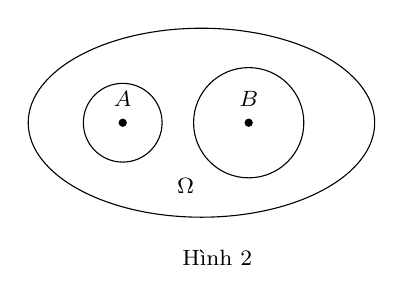
\begin{tikzpicture}[scale=1, font=\footnotesize, line join=round, line 
			cap=round, >=stealth]
			\path 
			(1.6,0) coordinate (B)
			(0,0) coordinate (A)
			(1,0) coordinate (C)
			;
			\draw (A) circle (0.5cm);
			\draw  (B) circle (0.7cm);
			\draw (C)  ellipse (2.2cm and 1.2cm) ;
			\draw (0.8,-0.8) node{$\Omega$}
			(1.2,-1.5)node[below]{Hình 2};
			\foreach \p/\r in {A/90,B/90}
			\fill (\p) circle (1.5pt) node[shift={(\r:3mm)}]{$\p$};
	\end{tikzpicture}}
\end{boxdn}

\begin{luuy}
	Chú ý: Hai biến cố $A$ và $B$ là xung khắc khi và chỉ khi $A \cap B=\varnothing$.
\end{luuy}
\subsubsection{Biến cố độc lập}
\indam{Định nghĩa:}
\begin{boxdn}
	Hai biến cố $A$ và $B$ được gọi là {\bf \textit{độc lập}} nếu việc xảy ra hay không xảy ra của biến cố này không làm ảnh hưởng tới xác suất xảy ra của biến cố kia.
\end{boxdn}
\begin{luuy}
	Nhận xét: Nếu hai biến cố $A$ và $B$ độc lập thì $\overline{A}$ và $B ; A$ và $\overline{B} ; \overline{A}$ và $\overline{B}$ cũng độc lập.
\end{luuy}
\subsubsection{Quy tắc nhân xác suất của hai biến cố độc lập}
\indam{Định nghĩa:}
\begin{boxdn}
	Nếu hai biến cố $A$ và $B$ độc lập thì
	$$\mathrm{P}(AB)=\mathrm{P}(A) \mathrm{P}(B).$$
\end{boxdn}
\begin{luuy}
	Chú ý: Từ quy tắc nhân xác suất ta thấy, nếu $\mathrm{P}(AB) \neq \mathrm{P}(A) \mathrm{P}(B)$ thì hai biến cố $A$ và $B$ không độc lập.
\end{luuy}
%-------------------------------------------------------------------------------------------------------------
\subsection{PHÂN LOẠI VÀ PHƯƠNG PHÁP GIẢI TOÁN}%3 ví dụ tự luận mỗi dạng
\begin{dang}{Xác định biến cố giao}
	Tập hợp mô tả biến cố $AB$ là giao của hai tập hợp mô tả biến cố $A$ và biến cố $B$.
\end{dang}
\begin{vd}[Sách bài tập Kết nối tri thức]%[1D2Y1-1]%[Dự án đề cương 3 Khối NH24-25-Dot 1-Nhật Thiện]
	Hai xạ thủ $X$, $Y$ mỗi người bắn một viên đạn vào một mục tiêu. Xét các biến cố $A$: \lq\lq Xạ thủ $X$ bắn trúng\rq\rq; $B$: \lq\lq Xạ thủ $Y$ bắn trúng\rq\rq.\\
	Nêu nội dung của các biến cố $AB$, $\overline{AB}$, $\overline{A}B$, $A\overline{B}$.
	\loigiai{		
		\begin{itemize}
			\item $AB$: \lq\lq Cả hai xạ thủ bắn trúng \rq\rq.
			\item $\overline{AB}$: \lq\lq Cả hai xạ thủ bắn trượt \rq\rq.
			\item $\overline{A}B$: \lq\lq Xạ thủ $X$ bắn trượt, xạ thủ $Y$ bắn trúng \rq\rq.
			\item $A\overline{B}$: \lq\lq Xạ thủ $X$ bắn trúng, xạ thủ $Y$ bắn trượt \rq\rq.
		\end{itemize}
	}
\end{vd}
\begin{vd}%[1D2Y1-3]%[Dự án đề cương 3 Khối NH24-25-Dot 1-Nhật Thiện]
	Gieo một xúc xắc cân đối và đồng chất hai lần liên tiếp. Xét các biến cố:
	\begin{enumerate}[ ]
		\item $A$: ``Số chấm xuất hiện ở lần gieo thứ nhất là số lẻ''.
		\item $B$: ``Số chấm xuất hiện ở lần gieo thứ hai là số lẻ''.
	\end{enumerate}
	Chọn phát biểu đúng trong các phát biểu sau đây:
	\begin{enumerate}
		\item Biến cố giao của hai biến cố $A$ và $B$ là ``Số chấm xuất hiện ở lần gieo thứ nhất là số lẻ hoặc số chấm xuất hiện ở lần gieo thứ hai là số lẻ''.
		\item Biến cố giao của hai biến cố $A$ và $B$ là ``Số chấm xuất hiện ở lần gieo thứ nhất là số lẻ và số chấm xuất hiện ở lần gieo thứ hai là số lẻ''.
		\item Biến cố giao của hai biến cố $A$ và $B$ là ``Tích số chấm xuất hiện ở hai lần gieo là số lẻ''.
		\item Biến cố giao của hai biến cố $A$ và $B$ là ``Tích số chấm xuất hiện ở hai lần gieo là số chẵn''.
	\end{enumerate}
	\loigiai{
		\begin{itemize}
			\item Phát biểu đúng là b) và c).
			\item Phát biểu sai là a) và d).
		\end{itemize}
	}
\end{vd}
\begin{vd}%[1D2Y1-3]%[Dự án đề cương 3 Khối NH24-25-Dot 1-Nhật Thiện]
	Gieo hai con xúc xắc cân đối và đồng chất. Gọi $A$ là biến cố \lq\lq Tổng số chấm xuất hiện trên hai con xúc xắc bằng 5\rq\rq, $B$ là biến cố \lq\lq Tích số chấm xuất hiện trên hai con xúc xắc bằng 6\rq\rq. Gọi $C$ là biến cố \lq\lq Có ít nhất một con xúc xắc xuất hiện mặt $1$ chấm\rq\rq. Hãy viết tập hợp mô tả các biến cố giao $AC$ và $BC$.
	\loigiai{
		Biến cố $A=\{(1 ; 4) ;(4 ; 1) ;(2 ; 3) ;(3 ; 2)\}$.\\
		Biến cố $B=\{(1 ; 6) ;(6 ; 1) ;(2 ; 3) ;(3 ; 2)\}$.\\
		Biến cố $C=\{(1 ; 6) ;(6 ; 1) ;(1 ; 5) ;(5 ; 1) ;(1 ; 4) ;(4 ; 1) ;(1 ; 3) ;(3 ; 1) ;(1 ; 2) ;(2 ; 1) ;(1 ; 1)\}$.\\
		Kết hợp tập hợp mô tả biến cố $A, B$ ở trên, ta có biến cố $AC=\{(1 ; 4) ;(4 ; 1)\};$  $B C=\{(1 ; 6) ;(6 ; 1)\}.$
		
	}
\end{vd}
\begin{dang}{Xác định biến cố xung khắc}
	Hai biến cố $A$ và $B$ được gọi là {\bf\textit{xung khắc}} nếu $A$ và $B$ không đồng thời xảy ra.\\
	Chú ý: Hai biến cố $A$ và $B$ là xung khắc khi và chỉ khi $A \cap B=\varnothing$.
\end{dang}
\begin{vd}[Sách giáo  khoa Cánh diều]%[1C5Y2-1]%[Dự án đề cương 3 Khối NH24-25-Dot 1-Nhật Thiện]
	Tung một đồng xu cân đối và đồng chất hai lần liên tiếp. Xét các biến cố:\\
	A: \lq\lq Đồng xu xuất hiện mặt $S$ ở lần gieo thứ nhất\rq\rq.\\
	B: \lq\lq Đồng xu xuất hiện mặt $N$ ở lần gieo thứ nhất\rq\rq.\\
	Hai biến cố trên có xung khắc không?\\
	\loigiai{
		Ta thấy	$A=\{S S ; S N\} ; B=\{N S ; N N\}$.\\
		Suy ra $A \cap B=\varnothing$. Do đó, $A$ và $B$ là hai biến cố xung khắc.
	}
\end{vd}
\begin{vd}%[1D2B1-3]%[Dự án đề cương 3 Khối NH24-25-Dot 1-Nhật Thiện]
	Tung một đồng xu cân đối và đồng chất ba lần liên tiếp. Xét các biến cố:
	\begin{enumerate}[]
		\item $A$: ``Đồng xu xuất hiện mặt sấp (S) ở lần tung thứ nhất''.
		\item $B$: ``Đồng xu xuất hiện mặt ngửa (N) ở lần tung thứ nhất''.
	\end{enumerate}
	Hai biến cố trên có xung khắc hay không?
	\loigiai{
		Ta có $\begin{aligned}[t]
			A&=\{\text{SSS;SSN;SNS;SNN}\}\\
			B&=\{\text{NSS;NSN;NNS;NNN}\}.
		\end{aligned}$\\
		Suy ra $A \cap B=\varnothing$. Do đó $A$ và $B$ là hai biến cố xung khắc.
	}
\end{vd}
\begin{vd}%[1D2B1-3]%[Dự án đề cương 3 Khối NH24-25-Dot 1-Nhật Thiện]
	Một hộp có $5$ viên bi xanh, $4$ viên bi đỏ và $2$ viên bi vàng. Lấy ra ngẫu nhiên đồng thời $2$ viên bi từ hộp. Hãy xác định các cặp biến cố xung khắc trong các biến cố sau:\\
	$A$ : \lq\lq Hai viên bi lấy ra cùng màu xanh\rq\rq;\\
	$B$ : \lq\lq Hai viên bi lấy ra cùng màu đỏ\rq\rq;\\
	$C$ : \lq\lq Hai viên bi lấy ra cùng màu\rq\rq;\\
	$D$ : \lq\lq Hai viên bi lấy ra khác màu\rq\rq.
	\loigiai{
		\begin{enumerate}
			\item Ta có hai biến cố $A$ và $B$ xung khắc.
			\item Biến cố $C$ xảy ra khi lấy ra 2 viên bi xanh hoặc 2 viên bi đỏ hoặc 2 viên bi vàng. Khi lấy được 2 viên bi màu xanh thì biến cố $A$ và biến cố $C$ cùng xảy ra. Khi lấy được 2 viên bi màu đỏ thì biến cố $B$ và biến cố $C$ cùng xảy ra. Do đó biến cố $C$ không xung khắc với biến cố $A$ và biến cố $B$.
			\item Biến cố $D$ xảy ra khi lấy ra 1 viên bi xanh, 1 viên bi đỏ; hoặc 1 viên bi xanh, 1 viên bi vàng; hoặc 1 viên bi đỏ, 1 viên bi vàng. Do đó biến cố $D$ xung khắc với biến cố $A$, xung khắc với biến cố $B$ và xung khắc với biến cố $C$.
		\end{enumerate}
		Vậy có 4 cặp biến cố xung khắc là: $A$ và $B ; A$ và $D ; B$ và $D ; C$ và $D$.
	}
\end{vd}
\begin{dang}{Xác định biến cố độc lập}
	
\end{dang}

\begin{vd}[Sách Bài tập Cánh diều]%[1D2K1-3]%[Dự án đề cương 3 Khối NH24-25-Dot 1-Nhật Thiện]
	Một hộp có 7 viên bi màu xanh và 8 viên bi màu đỏ, các viên bi có kích thước và khối lượng như nhau. Lấy viên bi ngẫu nhiên hai lần liên tiếp, trong đó mỗi lần lấy ngẫu nhiên một viên bi trong hộp, ghi lại màu của viên bi lấy ra và bỏ lại viên bi đó vào hộp. Xét các biến cố:
	\begin{enumerate}[]
		\item $A$: ``Viên bi màu đỏ được lấy ra ở lần thứ nhất''.
		\item $B$: ``Viên bi màu xanh được lấy ra ở lần thứ hai''.
	\end{enumerate}
	Hai biến cố $A$ và $B$ có độc lập không? Vì sao?
	\loigiai{
		Trước hết, xác suất của biến cố $B$ khi biến cố $A$ xảy ra bằng $\dfrac{7}{15}$, xác suất của biến cố $B$ khi biến cố $A$ không xảy ra cũng bằng $\dfrac{7}{15}$. \\
		Do đó việc xảy ra hay không xảy ra của biến cố $A$ không làm ảnh hưởng đến xác suất xảy ra của biến cố $B$. \\
		Mặt khác, xác suất của biến cố $A$ bằng $\dfrac{8}{15}$, không phụ thuộc vào việc xảy ra hay không xảy ra của biến cố $B$.\\
		Vậy hai biến cố $A$ và $B$ là độc lập.
	}
\end{vd}
\begin{vd}[Sách giáo khoa Cánh diều]%[1C5Y2-1]%[Dự án đề cương 3 Khối NH24-25-Dot 1-Nhật Thiện]
	Một hộp có $3$ quả bóng màu xanh, $4$ quả bóng màu đỏ; các quả bóng có kích thước và khối lượng như nhau. Lấy bóng ngẫu nhiên hai lần liên tiếp, trong đó mỗi lần lấy ngẫu nhiên một quả bóng trong hộp, ghi lại màu của quả bóng lấy ra và bỏ lại quả bóng đó vào hộp.\\
	Xét các biến cố:\\
	$A$: \lq\lq Quả bóng màu xanh được lấy ra ở lần thứ nhất\rq\rq;\\
	$B$: \lq\lq Quả bóng màu đỏ được lấy ra ở lần thứ hai\rq\rq.\\
	Hỏi
	\begin{enumerate}[a)]
		\item Hai biến cố $A$ và $B$ có độc lập không? Vì sao?
		\item Hai biến cố $A$ và $B$ có xung khắc không? Vì sao?
	\end{enumerate}
	\loigiai{
		\begin{enumerate}[a)]
			\item Trước hết, biến cố $B$ xảy ra sau biến cố $A$ nên việc xảy ra hay không xảy ra của biến cố $B$ không làm ảnh hưởng đến xác suất xảy ra của biến cố $A$.\\
			Mặt khác, ta có xác suất của biến cố $B$ khi biến cố $A$ xảy ra bằng $\dfrac{4}{7}$; xác suất của biến cố $B$ khi biến cố $A$ không xảy ra cũng bằng $\dfrac{4}{7}$.\\
			Do đó việc xảy ra hay không xảy ra của biến cố $A$ không làm ảnh hưởng đến xác suất xảy ra của biến cố $B$.\\
			Vậy hai biến cố $A$ và $B$ là độc lập.
			\item Ta thấy kết quả (xanh; đỏ) là kết quả thuận lợi cho cả hai biến cố $A$ và $B$. Vì thế $A$ và $B$ không là hai biến cố xung khắc.
	\end{enumerate}}		
\end{vd}
\begin{vd}[Sách Bài tập Kết nối tri thức]%[1D2Y1-1]%[Dự án đề cương 3 Khối NH24-25-Dot 1-Nhật Thiện]
	Có hai lọ hoa. Lọ $I$ cắm 5 bông hoa hồng và 3 bông hoa cúc. Lọ $II$ cắm 4 bông hoa hồng và 5 bông hoa thược dược. Lấy ngẫu nhiên đồng thời từ mỗi lọ một bông hoa. Xét hai biến cố sau:
	\begin{center}
		$A$: \lq\lq Lấy được bông hoa hồng từ lọ $I$\rq\rq, $B$: \lq\lq Lấy bông hoa hồng từ lọ $II$\rq\rq.
	\end{center}
	Chứng tỏ rằng $A$ và $B$ độc lập.  
	\loigiai{
		\begin{itemize}
			\item Dù $A$ có xảy ra (lấy được bông hoa hồng) hay $A$ không xảy ra (lấy được bông hoa cúc) ta đều có $\mathrm{P}(B)=\dfrac{4}{9}$.
			\item Dù $B$ có xảy ra (lấy được bông hoa hồng) hay $B$ không xảy ra (lấy được bông hoa thược dược) ta đều có $\mathrm{P}(A)=\dfrac{5}{8}$.
		\end{itemize}
		Việc xảy ra hay không xảy ra của biến cố này không ảnh hưởng tới xác suất xảy ra của biến cố kia. Vậy $A$ và $B$ độc lập.
	}
\end{vd}
\begin{dang}{Quy tắc nhân xác suất}
	
\end{dang}
\begin{vd}[Sách giáo  khoa Cánh diều]%[1C5B2-6]%[Dự án đề cương 3 Khối NH24-25-Dot 1-Nhật Thiện]
	Hai bạn Hạnh và Hà cùng chơi trò chơi bắn cung một cách độc lập. Mỗi bạn chỉ bắn một lần. Xác suất để bạn Hạnh và bạn Hà bắn trúng bia lần lượt là $0{,}6$ và $0{,}7$ trong lần bắn của mình. Tính xác suất của biến cố $C$: \lq\lq Bạn Hạnh và bạn Hà đều bắn trúng bia \rq\rq.
	\loigiai{
		Xét biến cố $A$: \lq\lq Bạn Hạnh bắn trúng bia\rq\rq, ta có $\mathrm{P}(A)=0{,}6$.\\
		Xét biến cố $B$: \lq\lq Bạn Hà bắn trúng bia\rq\rq, ta có $\mathrm{P}(B)=0{,}7$.\\
		Ta thấy $A, B$ là hai biến cố độc lập và $C=A \cap B$. suy ra
		$$\mathrm{P}(C)=\mathrm{P}(A) \cdot \mathrm{P}(B)=0{,}6 \cdot 0{,}7=0{,}42.$$}
\end{vd}
\begin{vd}[Sách bài tập Cánh diều]%[1D2K2-6]%[Dự án đề cương 3 Khối NH24-25-Dot 1-Nhật Thiện]
	Một xưởng sản xuất có hai động cơ chạy độc lập với nhau. Xác suất để động cơ I và động cơ II chạy tốt lần lượt là $0{,}7$ và $0{,}8$. Tính xác suất của biến cố $C$: ``Cả hai động cơ đều chạy tốt''.
	\loigiai{
		Xét biến cố $A$: ``Động cơ I chạy tốt'', ta có $\mathrm{P}(A)=0{,}7$.\\
		Xét biến cố $B$: ``Động cơ II chạy tốt'', ta có $\mathrm{P}(B)=0{,}8$.\\
		Ta thấy $A$ và $B$ là hai biến cố độc lập và $C=A \cap B$.\\
		Suy ra $\mathrm{P}(C)=\mathrm{P}(A \cap B)=\mathrm{P}(A) \cdot \mathrm{P}(B)=0{,}7 \cdot 0{,}8=0{,}56$.	
	}
\end{vd}
\begin{vd}[Sách bài tập Chân trời sáng tạo]%[1D9B1-4]%[Dự án đề cương 3 Khối NH24-25-Dot 1-Nhật Thiện]
	Cho $A$ và $B$ là hai biến cố độc lập.
	\begin{enumEX}[a)]{1}
		\item Biết $\mathrm{P}(A)=0{,}3$ và $\mathrm{P}(B)=0{,}7$. Hãy tính xác suất của các biến cố $AB$, $\overline{A}B$ và $\overline{A}\overline{B}$.
		\item Biết $\mathrm{P}(A)=0{,}8$ và $\mathrm{P}(AB)=0{,}4$. Hãy tính xác suất của các biến cố $B$, $\overline{A}B$ và $\overline{A}\overline{B}$.
	\end{enumEX}
	\loigiai{
		\begin{enumEX}[a)]{1}
			\item Do $A$ và $B$ là hai biến cố độc lập nên xác suât của biến cố $A B$ là
			$$\mathrm{P}(AB)=\mathrm{P}(A)\cdot \mathrm{P}(B)=0{,}3\cdot 0{,}7=0{,}21.$$
			Vì $\overline{A}$ là biến cố đối của $A$ nên $\mathrm{P}(\overline{A})=1-\mathrm{P}(A)=0{,}7$.\\
			Do $\overline{A}$ và $B$ là hai biến cố độc lập nên xác suất của biến cố $\overline{A} B$ là
			$$\mathrm{P}(\overline{A}B)=\mathrm{P}(\overline{A})\mathrm{P}(B)=0{,}7\cdot0{,}7=0{,}49.$$
			Vì $\overline{B}$ là biến cố đối của $B$ nên $\mathrm{P}(\overline{B})=1-\mathrm{P}(B)=0{,}3$.\\
			Do $\overline{A}$ và $\overline{B}$ là hai biến cố độc lập nên xác suất của biến cố $\overline{A} \overline{B}$ là
			$$\mathrm{P}(\overline{A}\overline{B})=\mathrm{P}(\overline{A})\cdot \mathrm{P}(\overline{B})=0{,}7\cdot0{,}3=0{,}21.$$
			\item Do $A$ và $B$ là hai biến cố độc lập nên
			$$\mathrm{P}(B)=\dfrac{\mathrm{P}(AB)}{\mathrm{P}(A)}=\dfrac{0{,}4}{0{,}8}=0{,}5.$$
			Vì $\overline{A}$ là biến cố đối của $A$ nên $\mathrm{P}(\overline{A})=1-\mathrm{P}(A)=0{,}2$.\\
			Do $\overline{A}$ và $B$ là hai biến cố độc lập nên xác suất của biến cố $\overline{A} B$ là
			$$\mathrm{P}(\overline{A}B)=\mathrm{P}(\overline{A})\cdot \mathrm{P}(B)=0{,}2\cdot0{,}5=0{,}1.$$
			Vì $\overline{B}$ là biến cố đối của $B$ nên $\mathrm{P}(\overline{B})=1-\mathrm{P}(B)=0{,}5$.\\
			Do $\overline{A}$ và $\overline{B}$ là hai biến cố độc lập nên xác suất của biến cố $\overline{A} \overline{B}$ là
			$$\mathrm{P}(\overline{A}\overline{B})=\mathrm{P}(\overline{A})\cdot \mathrm{P}(\overline{B})=0{,}2 \cdot 0{,}5=0{,}1.$$
		\end{enumEX}
	}
	
\end{vd}
\begin{dang}{Tính xác suất bằng sơ đồ hình cây}
	
\end{dang}
\begin{vd}[Sách bài tập Chân trời sáng tạo]%[1D9K1-3]%[Dự án đề cương 3 Khối NH24-25-Dot 1-Nhật Thiện]
	Minh gieo $1$ hạt đậu và $1$ hạt ngô. Xác suất nảy mầm của hạt đậu và hạt ngô lần lượt là $0{,}7$ và $0{,}6$. Biết rằng sự nảy mầm của hai hạt này là độc lập. Sử dụng sơ đồ hình cây, tính xác suất của các biến cố:
	\begin{enumEX}[a)]{1}
		\item \lq\lq Cả $2$ hạt đều nảy mầm\rq\rq;
		\item \lq\lq Cả $2$ hạt đều không nảy mầm\rq\rq;
		\item \lq\lq Hạt đậu nảy mầm, hạt ngô không nảy mầm\rq\rq.
	\end{enumEX}
	\loigiai{
		Ta có sơ đồ hình cây như sau:
		\begin{center}
			\begin{tikzpicture}[>=stealth,line cap=round,line join=round]
				\path
				(0,0)coordinate(O)
				(1,2)coordinate(A)
				(1,-2)coordinate(B)
				(3,2)coordinate(A1)
				(4,3)coordinate(A2)
				(4,1)coordinate(A2')
				(3,-2)coordinate(B1)
				(4,-1)coordinate(B2)
				(4,-3)coordinate(B2')
				(7,4)coordinate(C)node[right]{Kết quả}
				(7,3)coordinate(C1)node[above right]{Hạt đậu nảy mầm,}node[below right]{Hạt ngô nảy mầm}
				(7,1)coordinate(C2)node[above right]{Hạt đậu nảy mầm,}node[below right]{Hạt ngô không nảy mầm}
				(7,-1)coordinate(C3)node[above right]{Hạt đậu không nảy mầm,}node[below right]{Hạt ngô nảy mầm}
				(7,-3)coordinate(C4)node[above right]{Hạt đậu không nảy mầm,}node[below right]{Hạt ngô không nảy mầm}
				(11.5,4)coordinate(D)node[right]{Xác suất}
				(11.5,3)coordinate(D)node[right]{$0{,}42$}
				(11.5,1)coordinate(D)node[right]{$0{,}28$}
				(11.5,-1)coordinate(D)node[right]{$0{,}18$}
				(11.5,-3)coordinate(D)node[right]{$0{,}12$}
				;
				\draw[->](O)--(A)node[above right]{Hạt đậu}node[below right]{nảy mầm}node[midway,left]{$0{,}7$};
				\draw[->](A1)--(A2)node[above right]{Hạt ngô}node[below right]{nảy mầm}node[midway,left]{$0{,}6$};
				\draw[->](A1)--(A2')node[above right]{Hạt ngô}node[below right]{ không nảy mầm}node[midway,left]{$0{,}4$};
				\draw[->](O)--(B)node[above right]{Hạt đậu}node[ right]{không}node[below right]{nảy mầm}node[midway,left]{$0{,}3$};
				\draw[->](B1)--(B2)node[above right]{Hạt ngô}node[below right]{nảy mầm}node[midway,left]{$0{,}6$};
				\draw[->](B1)--(B2')node[above right]{Hạt ngô}node[below right]{không nảy mầm}node[midway,left]{$0{,}4$};
			\end{tikzpicture}
		\end{center}
		\begin{enumEX}[a)]{1}
			\item Xác suất cả $2$ hạt đều nảy mầm là $0{,}42$.
			\item Xác suất cả $2$ hạt đều không nảy mầm là $0{,}12$.
			\item Xác suất hạt đậu nảy mầm, hạt ngô không nảy mầm là $0{,}28$.	
		\end{enumEX}
	}
\end{vd}
\begin{vd}[Sách bài tập Cánh diều]%[1D2K2-3]%[Dự án đề cương 3 Khối NH24-25-Dot 1-Nhật Thiện]
	Một người cho ngẫu nhiên $3$ lá thư vào $3$ chiếc phong bì đã ghi địa chỉ sao cho mỗi phong bì chỉ chứa một lá thư. Tính xác suất để có ít nhất một lá thư được cho vào đúng phong bì đã ghi địa chỉ theo lá thư đó.
	\loigiai{
		Giả sử lá thư I, lá thư II, lá thư III tương ứng với các phong bì đã ghi đúng địa chỉ là phong bì I, phong bì II, phong bì III.\\
		Mỗi cách chọn $3$ phong bì cho $3$ lá thư tương ứng với một hoán vị của $3$ phần tử. Do đó số phần tử của không gian mẫu là $n(\Omega)=3!=6$.\\
		Gọi $A$ là biến cố có ít nhất một lá thư được cho vào đúng phong bì đã ghi địa chỉ theo lá thư đó.\\
		Khi đó biến cố đối của biến cố $A$ là $\overline{A}$: ``Cả ba lá thư được cho vào phong bì không đúng địa chi''.\\
		Sơ đồ hình cây biểu thị các khả năng thuận lợi cho biến cố $\overline{A}$.
		\begin{center}
			\begin{tikzpicture}[>=stealth,line join=round,line cap=round,font=\footnotesize,scale=1]
				\tikzset{every node/.style={text width=5cm,draw,align=center}}
				\path
				(0,0) node(A){Cả ba lá thư cho vào phong bì không đúng địa chỉ}
				++(-10:6) node(B){Cho lá thư I vào phong bì III}
				++(-90:1)node(C){Cho lá thư II vào phong bì I}
				++(-90:1)node(D){Cho lá thư III vào phong bì II}
				($(A)+(-170:6)$)node(E){Cho lá thư I vào phong bì II}
				++(-90:1)node(F){Cho lá thư II vào phong bì III}
				++(-90:1)node(G){Cho lá thứ III vào phong bì I}
				;
				\foreach \a/\b in {A/B,B/C,C/D,A/E,E/F,F/G}\draw[->,double,red] (\a)--(\b);
			\end{tikzpicture}
		\end{center}
		Suy ra $n(\overline{A})=1+1=2$. Khi đó
		\[\mathrm{P}(\overline{A})=\dfrac{n(\overline{A})}{n(\Omega)}=\dfrac{2}{6}=\dfrac{1}{3} \Rightarrow \mathrm{P}(A)=1-\mathrm{P}(\overline{A})=1-\dfrac{1}{3}=\dfrac{2}{3}. \]
	}
\end{vd}
\begin{vd}[Sách bài tập Cánh diều]%[1D2K2-3]%[Dự án đề cương 3 Khối NH24-25-Dot 1-Nhật Thiện]
	Một hộp chứa $9$ quả cầu có cùng kích thước và khối lượng, trong đó có 4 quả cầu màu xanh đánh số từ 1 đến 4, có 3 quả cầu màu vàng đánh số từ 1 đến 3, có 2 quả cầu màu đỏ đánh số 1 và 2. Lấy ngẫu nhiên 2 quả cầu từ hộp. Tính xác suất để 2 quả cầu được lấy vừa khác màu vừa khác số.
	\loigiai{
		Mỗi cách lấy ngẫu nhiên 2 quả cầu từ một hộp có 9 quả cầu cho ta một tổ hợp chập 2 của 9 phần tử. Do đó không gian mẫu $\Omega$ gồm các tổ hợp chập 2 của 9 phần tử và $n(\Omega)=\mathrm{C}_9^2=36$.\\
		Xét biến cố $A$: ``Lấy được 2 quả cầu vừa khác màu vừa khác số''.
		Sơ đồ hình cây biểu thị các khả năng thuận lợi cho biến cố $A$
		\begin{center}
			\begin{tikzpicture}[>=stealth,line join=round,line cap=round,font=\footnotesize,scale=1]
				\tikzset{every node/.style={text width=4cm,draw,align=center}}
				\path
				(0,0) node(O){Lấy được 2 quả cầu vừa khác màu vừa khác số}
				++(-10:6) node(A){Lấy một quả màu vàng và một quả màu xanh}
				++(-90:1.5)node(B){Lấy quả màu vàng: có 3 cách chọn}
				++(-90:1.5)node(C){Lấy quả màu xanh: có 3 cách chọn}
				($(O)+(-170:6)$)node(D){Lấy một quả màu đỏ và một quả màu vàng}
				++(-90:1.5)node(E){Lấy quả màu đỏ: có 2 cách chọn}
				++(-90:1.5)node(F){Lấy quả màu vàng: có 2 cách chọn}
				($(O)+(-90:1.5)$)node(M){Lấy một quả màu đỏ và một quả màu xanh}
				++(-90:1.5)node(N){Lấy quả màu đỏ: có 2 cách chọn}
				++(-90:1.5)node(P){Lấy quả màu xanh: có 2 cách chọn}
				;
				\foreach \a/\b in {O/A,A/B,B/C,O/D,D/E,E/F,O/M,M/N,N/P}\draw[->,double,red] (\a)--(\b);
			\end{tikzpicture}
		\end{center}
		Suy ra $n(A)=2\cdot 2+2 \cdot 3+3\cdot 3=19$.\\
		Vậy $\mathrm{P}(A)=\dfrac{n(A)}{n(\Omega)}=\dfrac{19}{36}$.
	}
\end{vd}
%-----------------------------------------------------------------------------
\subsection{Bài tập rèn luyện}
\ind{PHẦN I.} \inden{Câu trắc nghiệm nhiều phương án lựa chọn. Mỗi câu hỏi học sinh chỉ chọn một phương án.}\\%20 CÂU
\setcounter{ex}{0}
\Opensolutionfile{ans}[ans/1T1-Bai1-TN]%--Đặt tên 2D1-Bai1-Dang1-TN
\begin{ex}%[1D2Y2-2]%[Dự án đề cương 3 Khối NH24-25-Dot 1-Nhật Thiện]
	Trên giá sách có các quyển vở không nhãn xếp cạnh nhau với bề ngoài, khối lượng và kích thước giống hệt nhau, trong đó có $5$ quyển ghi môn Toán, $5$ quyển ghi môn Ngữ Văn và $3$ quyển ghi môn Tiếng Anh. Lấy ngẫu nhiên hai quyển vở. Xét các biến cố:\\
	$M$: "Trong hai quyển vở được lấy, chỉ có $1$ quyển ghi môn Tiếng Anh";\\
	$N$ : "Trong hai quyển vở được lấy, chỉ có $1$ quyển ghi môn Ngữ Văn".\\
	Khi đó, biến cố giao của hai biến cố $M$ và $N$ là:
	\choice
	{ "Hai quyển vở được lấy ghi cùng một môn"}
	{ "Hai quyển vở được lấy ghi hai môn khác nhau"}
	{ \True "Trong hai quyển vở được lấy, một quyển ghi môn Tiếng Anh và một quyển ghi môn Ngữ Văn"}
	{ "Hai quyển vở được lấy có ít nhất một quyển ghi môn Tiếng Anh"}
	\loigiai{
	Ta cần lấy sao cho vừa chỉ có $1$ quyển ghi môn Tiếng Anh và chỉ có $1$ quyển ghi môn Ngữ Văn. Khi đó, trong hai quyển lấy ra chỉ có thể một Tiếng Anh và một Ngữ Văn.
}
\end{ex}
\begin{ex}%[1D9N1-1]%[Dự án đề cương 3 Khối NH24-25-Dot 1-Nhật Thiện]
	Gieo ngẫu nhiên một con xúc sắc cân đối và đồng chất hai lần liên tiếp. $A$ là biến cố \lq\lq Số chấm xuất hiện ở lần thứ nhất là số lẻ\rq\rq, $B$ là biến cố \lq\lq Số chấm xuất hiện ở lần thứ hai là số lẻ\rq\rq. Chọn khẳng định đúng.
	\choice
	{Hai biến cố $A$ và $B$ xung khắc}
	{$A$ và $B$ là hai biến cố đối nhau}
	{Biến cố giao của hai biến cố $A$ và $B$ là \lq\lq Số chấm xuất hiện ở lần thứ nhất hoặc lần thứ hai là số lẻ\rq\rq}
	{\True Biến cố giao của hai biến cố $A$ và $B$ là \lq\lq Số chấm xuất hiện hai lần gieo đều là số lẻ\rq\rq}
	\loigiai{
		$A \cap B$ là \lq\lq Số chấm xuất hiện ở lần thứ nhất là số lẻ và số chấm xuất hiện ở lần thứ hai là số lẻ\rq\rq.
	}
\end{ex}
\begin{ex}[\textit{Trích đề thi GHKII THPT Edison - Hải Phòng-Năm học 24-25}]%[1D9N1-1]%[Dự án đề cương 3 Khối NH24-25-Dot 1-Nhật Thiện]
	Cho hai biến cố $A$ và $B$. Nếu việc xảy ra hay không xảy ra của biến cố này không ảnh hưởng đến xác suất xảy ra của biến cố kia, thì hai biến cố $A$ và $B$ được gọi là?  
	\choice
	{Không giao với nhau}  
	{Biến cố đối của nhau}  
	{Xung khắc với nhau}  
	{\True Độc lập với nhau}  
	\loigiai{  
		Hai biến cố $A$ và $B$ được gọi là độc lập với nhau nếu xác suất xảy ra của $A$ không bị ảnh hưởng bởi việc xảy ra hay không xảy ra của $B$ và ngược lại.%\\
		%Điều này có nghĩa là  
		%\[
		%\mathrm{P}(A|B)=\mathrm{P}(A) \quad \text{và} \quad \mathrm{P}(B|A)=%\mathrm{P}(B)
		%\]
	}  
\end{ex}
\begin{ex}[\textit{Trích đề GHKII THPT Lê Quý Đôn - Ninh Thuận- Năm học 24-25}]%[1D9N1-2]%[Dự án đề cương 3 Khối NH24-25-Dot 1-Nhật Thiện]
	Chọn ngẫu nhiên một học sinh trong trường THPT chuyên Lê Quý Đôn. Gọi biến cố $A$: \lq\lq Học sinh được chọn bị cận thị \rq\rq và biến cố $B$: \lq\lq Học sinh được chọn học giỏi môn Toán\rq\rq. Xác định biến cố $AB$.
	\choice
	{\True Học sinh được chọn vừa bị cận thị vừa học giỏi môn Toán}
	{Học sinh được chọn học giỏi môn Toán nhưng không bị cận thị}
	{Học sinh được chọn bị cận thị nhưng không học giỏi môn Toán}
	{Học sinh được chọn bị cận thị hoặc học giỏi môn Toán}
	\loigiai{
		Biến cố $AB$ là: \lq\lq Học sinh được chọn vừa bị cận thị vừa học giỏi môn Toán.\rq\rq
	}
\end{ex}
\begin{ex}[\textit{Trích đề KT CKII THPT Nguyễn Tất Thành - Năm học 24-25}]%[1D9H1-2]%[Dự án đề cương 3 Khối NH24-25-Dot 1-Nhật Thiện]
	Một hộp chứa $21$ tấm thẻ cùng loại được đánh số thứ tự từ $1$ đến $21$. Chọn ra ngẫu nhiên $1$ thẻ từ hộp. Gọi $C$ là biến cố \lq\lq Số ghi trên thẻ được chọn chia hết cho $2$\rq\rq, $D$ là biến cố \lq\lq Số ghi trên thẻ được chọn chia hết cho $3$\rq\rq. Khi đó biến cố $CD$ là
	\choice
	{\lq\lq Số ghi trên thẻ được chọn chia hết cho $4$\rq\rq}
	{\lq\lq Số ghi trên thẻ được chọn chia hết cho $12$\rq\rq}
	{\lq\lq Số ghi trên thẻ được chọn chia hết cho $5$\rq\rq}
	{\True \lq\lq Số ghi trên thẻ được chọn chia hết cho $6$\rq\rq}
	\loigiai{
		Biến cố $CD$ là \lq\lq Số ghi trên thẻ được chọn chia hết cho $6$\rq\rq.
	}
\end{ex}
\begin{ex}%[1D9V2-3]%[Dự án đề cương 3 Khối NH24-25-Dot 1-Nhật Thiện]
	Một hộp chứa $15$ tấm thẻ cùng loại được đánh số từ $1$ đến $15$. Chọn ra ngẫu nhiên $1$ thẻ từ hộp. Gọi $A$ là biến cố \lq\lq Số ghi trên thẻ được chọn là số lẻ\rq\rq, biến cố nào sau đây là biến cố xung khắc với biến cố $A$?
	\choice
	{Số ghi trên thẻ được chọn nhỏ hơn $10$}
	{Số ghi trên thẻ được chọn chia hết cho $3$}
	{Số ghi trên thẻ được chọn chia hết cho $5$}
	{\True Số ghi trên thẻ được chọn chia hết cho $4$}
	\loigiai{
		Ta có $A=\{1;3;5;7;9;11;13;15\}$.\\
		Số ghi trên thẻ được chọn nhỏ hơn $10$ là $\{1; 2; 3; 4; 5; 6; 7; 8; 9\}$.\\
		Số ghi trên thẻ được chọn chia hết cho $3$ là $\{3;6;9;12;15\}$.\\
		Số ghi trên thẻ được chọn chia hết cho $5$ là $\{5;10;15\}$.\\
		Số ghi trên thẻ được chọn chia hết cho $4$ là $\{4;8;12\}$.\\
		Do đó biến cố xung khắc với biến cố $A$ là \lq\lq Số ghi trên thẻ được chọn chia hết cho $4$\rq\rq.}
\end{ex}
\begin{ex}%[1D9H1-1]%[Dự án đề cương 3 Khối NH24-25-Dot 1-Nhật Thiện]
	Gieo một con xúc xắc cân đối và đồng chất $2$ lần. Xét các biến cố:
	$A$: \lq\lq Số chấm xuất hiện trong hai lần gieo đều là số lẻ\rq\rq.
	$B$: \lq\lq Số chấm xuất hiện trong hai lần gieo đều là số chẵn\rq\rq.
	$C$: \lq\lq Số chấm xuất hiện trong lần gieo thứ nhất là $2$ \rq\rq.
	Khẳng định nào sau đây là \textbf{sai}?
	\choice
	{Hai biến cố $A$ và $B$ xung khắc}
	{Hai biến cố $A$ và $C$ xung khắc}
	{Hai biến cố $B$ và $C$ không xung khắc}
	{\True Hai biến cố $B$ và $C$ xung khắc}
	\loigiai{
		Ta có
		$A=\{(1,1);(1,3);(1,5);(3,1);(3,3);(3,5);(5,1);(5,3);(5,5)\}$.\\
		$B=\{(2,2);(2,4);(2,6);(4,2);(4,4);(4,6);(6,2);(6,4);(6,6)\}$.\\
		$C=\{(2,1);(2,2);(2,3);(2,4);(2,5);(2,6)\}$.\\
		Khi đó\\
		$AB=\varnothing$ nên $A$ và $B$ xung khắc.\\
		$AC=\varnothing$ nên $A$ và $C$ xung khắc.\\
		$BC=\{(2,2);(2,4);(2,6)\}$ nên $B$ và $C$ không xung khắc.
	}
\end{ex}
\begin{ex}[\textit{Trích đề kiểm tra Toán 11 HKII - THPT Chế Lan Viên - Năm học 24-25}]%[1D9H1-2]%[Dự án đề cương 3 Khối NH24-25-Dot 1-Nhật Thiện]
	Hộp thứ nhất đựng $4$ bi xanh được đánh số lần lượt từ $1$ đến $4$. Hộp thứ hai đựng $3$ bi đỏ được đánh số lần lượt từ $1$ đến $3$. Lấy ra ngẫu nhiên từ mỗi hộp một viên bi. Gọi
	$A$ là biến cố \lq \lq Tổng các số ghi trên $2$ bi là $5$\rq \rq, 
	$B$ là biến cố \lq \lq Tích các số ghi trên $2$ bi là số chẵn\rq \rq. Hãy viết tập hợp mô tả biến cố $AB$.
	\choice
	{$AB=\left\{(2;1);(2;3);(3;2);(4;1)\right\}$}
	{$AB=\left\{(1;2);(2;1);(2;2);(2;3);(3;2);(4;1);(4;2);(4;3)\right\}$}
	{\True $AB=\left\{(2;3);(3;2);(4;1)\right\}$}
	{$AB=\left\{(2;3);(3;2);(4;1);(4;2)\right\}$}
	\loigiai{Ta có
		$A=\left\{(2;3);(3;2);(4;1)\right\}$.\\
		$B=\left\{(1;2);(2;1);(2;2);(2;3);(3;2);(4;1);(4;2);(4;3)\right\}$.\\
		Do đó $AB=\left\{(2;3);(3;2);(4;1)\right\}$.
	}
\end{ex}
\begin{ex}[\textit{Trích đề HKII THPT Lương Thế Vinh - Hà Nội- Năm học 24-25}]%[1D9N1-3]%[Dự án đề cương 3 Khối NH24-25-Dot 1-Nhật Thiện]
	Cho $A$ và $B$ là hai biến cố độc lập. Biết rằng $\mathrm{P}(A)=0{,}4$ và $\mathrm{P}(B)=0{,}3$, xác suất của biến cố $AB$ bằng
	\choice
	{$0{,}58$}
	{$0{,}7$}
	{\True $0{,}12$}
	{$0{,}1$}
	\loigiai{
		Vì $A$ và $B$ là hai biến cố độc lập nên xác suất của biến cố $AB$ là
		$$ \mathrm{P}(AB)=\mathrm{P}(A)\cdot\mathrm{P}(B)=0{,}4\cdot 0{,}3=0{,}12. $$
	}
\end{ex}
\begin{ex}[\textit{Trích đề kiểm tra Toán 11 GHKII - THPT Trần Quang Khải - Năm học 24-25}]%[1D9N1-1]%[Dự án đề cương 3 Khối NH24-25-Dot 1-Nhật Thiện]
	Cho hai biến cố $A$ và $B$ độc lập. Chọn khẳng định đúng.
	\choice
	{$\mathrm{P}(A \cap B)=\mathrm{P}(B) -\mathrm{P}(A)$}
	{\True $\mathrm{P}(A \cap B)=\mathrm{P}(A)\cdot \mathrm{P}(B)$}
	{$\mathrm{P}(A \cap B)=\mathrm{P}(A) - \mathrm{P}(B)$}
	{$\mathrm{P}(A \cap B)=\mathrm{P}(A) + \mathrm{P}(B)$}
	\loigiai{
		Do hai biến cố $A$ và $B$ độc lập nên $\mathrm{P}(A \cap B)=\mathrm{P}(A)\cdot \mathrm{P}(B)$.
	}
\end{ex}
\begin{ex}[\textit{Trích đề kiểm tra Toán 11 HK2 -THPT Chuyên Trần Đại Nghĩa - NH24-25}]%[1D9H1-3]%[Dự án đề cương 3 Khối NH24-25-Dot 1-Nhật Thiện]
	Cho $A$ và $B$ là hai biến cố độc lập với nhau, biết $\mathrm{P}(A)=0{,}2$, $\mathrm{P}(B)=0{,}4$. Khi đó $\mathrm{P}(AB)$ bằng:
	\choice
	{\True $0{,}08$}
	{$0{,}8$}
	{$0{,}5$}
	{$0{,}6$}
	\loigiai{
		Vì $A$ và $B$ là hai biến cố độc lập, nên $\mathrm{P}(AB)=\mathrm{P}(A) \cdot \mathrm{P}(B)$.\\
		$\mathrm{P}(AB)=0{,}2 \cdot 0{,}4=0{,}08$.
	}
\end{ex}
\begin{ex}[\textit{Trích đề kiểm tra Toán 11 Cuối HK2 - THPT Nguyễn Tất Thành - Năm học 2024 2025}]%[1D9H1-2]%[Dự án đề cương 3 Khối NH24-25-Dot 1-Nhật Thiện]
	Cho $A$, $B$ là hai biến cố độc lập. Biết $\mathrm{P}(A)=0{,}3$; $\mathrm{P}(B)=0{,}7$. Xác suất của biến cố $AB$ là
	\choice
	{$0{,}21$}
	{$1$}
	{$0{,}49$}
	{$0{,}09$}
	\loigiai{
		Do $A$, $B$ là hai biến cố độc lập nên $\mathrm{P}(AB)=\mathrm{P}(A)\cdot \mathrm{P}(B)=0{,}3 \cdot 0{,}7=0{,}21$.
	}
\end{ex}
\begin{ex}%[1D9N1-3]%[Dự án đề kiểm tra Toán HKII NH24-25 - Đợt 11 - Hieu Phan]%[THPT Lý Thái Tổ - Bắc Ninh]%[Dự án đề cương 3 Khối NH24-25-Dot 1-Nhật Thiện]
	Cho $A$, $B$ là hai biến cố độc lập thỏa mãn $\mathrm{P}(A)=0{,}3$ và $\mathrm{P}(AB)=0{,}06$. Khi đó, $\mathrm{P}(\overline{B})$ bằng
	\choice
	{$0{,}6$}
	{$0{,}15$}
	{\True $0{,}8$}
	{$0{,}2$}
	\loigiai{
		Vì $A$ và $B$ là hai biến cố độc lập nên $$\mathrm{P}(AB)=\mathrm{P}(A) \cdot \mathrm{P}(B)\Leftrightarrow \mathrm{P}(B)=\dfrac{0{,}06}{0{,}3}=0{,}2.$$
		Xác suất của biến cố đối $\mathrm{P}(\overline{B})=1 - \mathrm{P}(B)=1 - 0{,}2=0{,}8$.
	}
\end{ex}
\begin{ex}%[Vũ Hồng Toàn]%[1D2B2-4]%[Dự án đề cương 3 Khối NH24-25-Dot 1-Nhật Thiện]
	Hai bạn Sơn và Tùng độc lập với nhau, mỗi người tung một con xúc xắc. Xác suất để xúc xắc của bạn Sơn xuất hiện số lẻ, xúc xắc của bạn Tùng xuất hiện số lớn hơn $4$ là
	\choice
	{\True $\dfrac{1}{6}$}
	{$\dfrac{1}{5}$}
	{$\dfrac{1}{7}$}
	{$\dfrac{2}{11}$}
	\loigiai{
		Gọi $A$ là biến cố: \lq\lq xúc xắc của bạn Sơn xuất hiện số lẻ\rq\rq,\\
		$B$ là biến cố: \lq\lq xúc xắc của bạn Tùng xuất hiện số lớn hơn $4$\rq\rq.\\
		$AB$ là biến cố: \lq\lq xúc xắc của bạn Sơn xuất hiện số lẻ và xúc xắc của bạn Tùng xuất hiện số lớn hơn 4\rq\rq.\\
		Ta có $\mathrm{P}(A)=\dfrac{n(A)}{n(\Omega)}=\dfrac{3}{6}=\dfrac{1}{2}$;  $\mathrm{P}(B)=\dfrac{n(B)}{n(\Omega)}=\dfrac{2}{6}=\dfrac{1}{3}$.\\
		Vì hai bạn Sơn và Tùng độc lập với nhau, mỗi người tung một con xúc xắc nên
		$$\mathrm{P}(AB)=\mathrm{P}(A)\cdot  \mathrm{P}(B)=\dfrac{1}{6}.$$
	}
\end{ex}
\begin{ex}%[1D9H1-3]%[Dự án đề cương 3 Khối NH24-25-Dot 1-Nhật Thiện]
	Hai xạ thủ độc lập bắn vào bia. Xác suất người thứ nhất bắn trúng bia là $0{,}6$; người thứ hai bắn trúng bia là $0{,}9$. Hãy tính xác suất để hai người cùng bắn trúng bia.
	\choice
	{$0{,}9$}
	{\True $0{,}54$}
	{$0{,}44$}
	{$0{,}6$}
	\loigiai{
		Gọi $A$ là biến cố \lq\lq người thứ nhất bắn trúng bia\rq\rq, $B$ là biến cố \lq\lq người thứ hai bắn trúng bia\rq\rq.\\
		Ta có $\mathrm{P}(A)=0{,}6$, $\mathrm{P}(B)=0{,}9$.\\
		Vì hai xạ thủ bắn độc lập nên $\mathrm{P}(A \cap B)=\mathrm{P}(A) \cdot \mathrm{P}(B)=0{,}6 \cdot 0{,}9=0{,}54$.
	}
\end{ex}
\begin{ex}[\textit{Trích đề kiểm tra Toán khối 11 HKII - THPT Ngô Quyền - Năm học 2024-2025}]%[1D9N1-1]%[Dự án đề cương 3 Khối NH24-25-Dot 1-Nhật Thiện]
	Cho hai biến cố $A$ và $B$ có $\mathrm{P}(A)=\dfrac{1}{3}$, $\mathrm{P}(B)=\dfrac{1}{4}$, $\mathrm{P}(AB)=\dfrac{1}{2}$. Kết luận nào sau đây đúng về hai biến cố $A$ và $B$?
	\choice
	{Độc lập}
	{\True Không độc lập}
	{Xung khắc}
	{Đối nhau}
	\loigiai{Ta có $\mathrm{P}(A)\cdot \mathrm{P}(B)=\dfrac{1}{3}\cdot\dfrac{1}{4}=\dfrac{1}{12}\neq \dfrac{1}{2}=\mathrm{P}(AB)$ nên hai biến cố $A$ và $B$ không độc lập.}
\end{ex}
\begin{ex}[\textit{Trích đề kiểm tra kì II khối 11 HKII - THPT Thuận Thanh 1 - Năm học 2024-2025}]%[1D9N1-3]%[Dự án đề cương 3 Khối NH24-25-Dot 1-Nhật Thiện]
	Cho $A$ và $B$ là hai biến cố. Biết $\mathrm{P}(A)=0{,}3$; $\mathrm{P}(B)=0{,}2$; $\mathrm{P}(AB)=0{,}06$. Khẳng định nào sau đây đúng?
	\choice
	{$A$ và $B$ là hai biến cố xung khắc}
	{$A$ và $B$ là hai biến cố không độc lập}
	{$A$ và $B$ là hai biến cố đối}
	{\True $A$ và $B$ là hai biến cố độc lập}
	\loigiai{
		Ta có  $\mathrm{P}(A) \cdot \mathrm{P}(B)=0{,}3 \cdot 0{,}2=0{,}06$ 
		mà $\mathrm{P}(AB)=0{,}06$ nên 
		$\mathrm{P}(AB)=\mathrm{P}(A) \cdot \mathrm{P}(B)$.\\
		Suy ra $A$ và $B$ là hai biến cố độc lập.		
	}
\end{ex}
\begin{ex}%[1D2B2-4]%[Dự án đề cương 3 Khối NH24-25-Dot 1-Nhật Thiện]
	Một trường học có hai máy in $A$ và $B$ hoạt động độc lập. Trong $24$ giờ hoạt động, xác suất để máy $A$ và máy $B$ gặp lỗi kĩ thuật tương ứng là $0{,}08$ và $0{,}12$. Xác suất để trong $24$ giờ hoạt động có nhiều nhất một máy gặp lỗi kĩ thuật là
	\choice
	{$0{,}99$}
	{\True $0{,}9904$}
	{$0{,}991$}
	{$0{,}9906 $}
	\loigiai{
		Gọi $M$ là biến cố: \lq\lq Máy in $A$ gặp lỗi kĩ thuật trong $24$ giờ hoạt động\rq\rq.\\
		$N$ là biến cố: \lq\lq Máy in $B$ gặp lỗi kĩ thuật trong $24$ giờ hoạt động\rq\rq.\\
		$H$ là biến cố: \lq\lq Trong $24$ giờ hoạt động có nhiều nhất một máy gặp lỗi kĩ thuật\rq\rq.\\
		Khi đó $\overline {H}$ là biến cố: \lq\lq Trong $24$ giờ hoạt động cả hai máy đều gặp lỗi kĩ thuật\rq\rq.\\
		$\overline{H}=MN \Rightarrow \mathrm{P}(MN)=\mathrm{P}(M) \cdot \mathrm{P}(N)=0{,}08 \cdot 0{,}12=0{,}0096$.\\
		Vậy $\mathrm{P}(H)=1-\mathrm{P}(\overline{H})=1-0{,}0096=0{,}9904$.
	}
\end{ex}
\begin{ex} %[1D2Y2-4]%[Dự án đề cương 3 Khối NH24-25-Dot 1-Nhật Thiện]
	Một hộp đựng 10 viên bi đỏ được đánh số từ $1$ đến $10$ và $15$ viên bi xanh được đánh số từ $1$ đến $15$ . Các viên bi có cùng kích thước và khối lượng. Lấy ra ngẫu nhiên $1$ viên bi từ trong hộp. Gọi $A$ là biến cố "Viên bi lấy ra có màu đỏ", $B$ là biến cố "Viên bi lấy ra ghi số chẵn". Xác suất của biến cố $A B$ là
	\choice
	{$0,28$}
	{\True $0,2$}
	{$0,4$}
	{$0,48$}
	\loigiai{
		Ta có $AB$ là biến cố "Viên bi lấy ra màu đỏ và ghi số chẵn".\\
		Vậy $$\mathrm{P}(AB)=\dfrac{5}{25}=0,2.$$	
	}
\end{ex}
\begin{ex}%[1D9H1-3]%[Dự án đề cương 3 Khối NH24-25-Dot 1-Nhật Thiện]
	Một chiếc máy có hai động cơ I và II hoạt động độc lập với nhau. Xác suất để động cơ I và II bị hỏng lần lượt là $0{,}4$ và $0{,}3$. Xác suất của biến cố \lq\lq Cả hai động cơ đều chạy tốt\rq\rq \ là
	\choice
	{$ 0{,}12 $}
	{$ 0{,}18 $}
	{\True $ 0{,}42 $}
	{$ 0{,}28 $}
	\loigiai{
		Xác suất động cơ I hoạt động tốt là  $1 - 0{,}4=0{,}6$.\\
		Xác suất động cơ II hoạt động tốt là $1 - 0{,}3=0{,}7$.\\
		Gọi $ X $ là biến cố  \lq\lq Cả hai động cơ đều chạy tốt\rq\rq \ và do độc lập nên
		$$\mathrm{P}(X)=0{,}6 \cdot 0{,}7=0{,}42.$$
	}
\end{ex}
\Closesolutionfile{ans}

\ind{PHẦN II.} \inden{Câu trắc nghiệm đúng sai. Trong mỗi ý a), b), c), d) ở mỗi câu, học sinh chọn đúng hoặc sai.}\\%5 CÂU
\setcounter{ex}{0}
\Opensolutionfile{ans}[ans/1T1-Bai1-DS]%--Đặt tên 2D1-Bai1-DS
\begin{ex}%[1D9H1-2]%[Dự án đề cương 3 Khối NH24-25-Dot 1-Nhật Thiện]
	Có hai chuồng nuôi gà. Chuồng I có $5$ con gà trống và $10$ con gà mái. Chuồng II có $3$ con gà mái và $7$ con gà trống. Từ mỗi chuồng bắt ngẫu nhiên một con gà. Gọi:
	\begin{itemize}
		\item $A$ là biến cố: \lq\lq bắt được gà mái từ chuồng I\rq\rq;
		\item $B$ là biến cố: \lq\lq bắt được gà trống từ chuồng II\rq\rq;
	\end{itemize}
	Khi đó
	\choiceTF
	{\True $n(A)=10$}
	{$n(B)=5$}
	{$\mathrm{P}(A)=\dfrac{1}{3}$ và $\mathrm{P}(B)=\dfrac{7}{10}$}
	{\True Hai biến cố $A$ và $B$ là độc lập}
	\loigiai{
		\begin{itemchoice}
			\itemch  $n(A)=10$.
			\itemch  $n(B)=3$.
			\itemch Ta có $\mathrm{P}(A)=\dfrac{10}{15}=\dfrac{2}{3}$ và $\mathrm{P}(B)=\dfrac{7}{10}$.
			\itemch  Dù $B$ xảy ra hay không xảy ra thì $\mathrm{P}(A)=\dfrac{2}{3}$.\\
			Dù $A$ xảy ra hay không xảy ra thì $\mathrm{P}(B)=\dfrac{7}{10}$.\\
			Vậy hai biến cố $A$ và $B$ là độc lập.
		\end{itemchoice}
	}
\end{ex}
\begin{ex}%[1D9H1-2]%[Dự án đề cương 3 Khối NH24-25-Dot 1-Nhật Thiện]
	Một hộp đựng $20$ tấm thẻ cùng loại được đánh số từ $1$ đến $20$. Rút ngẫu nhiên một tấm thẻ trong hộp. Gọi:
	\begin{itemize}
		\item $A$ là biến cố: \lq\lq Số ghi trên tấm thẻ là số chia hết cho $4$\rq\rq;
		\item $B$ là biến cố: \lq\lq Số ghi trên tấm thẻ là số nguyên tố\rq\rq;
		\item $C$ là biến cố: \lq\lq Số ghi trên tấm thẻ chia hết cho $6$\rq\rq.
	\end{itemize}
	Khi đó
	\choiceTF
	{$A=\{4; 8; 12; 16; 20\}$, $B=\{3; 5; 7; 11; 13; 17; 19\}$, $C=\{6; 12; 18\}$}
	{\True $A$ và $B$ là hai biến cố xung khắc}
	{\True $B$ và $C$ là hai biến cố xung khắc}
	{$A$ và $C$ là hai biến cố xung khắc}
	\loigiai{
		\begin{itemchoice}
			\itemch Ta có $A=\{4; 8; 12; 16; 20\}$, $B=\{2; 3; 5; 7; 11; 13; 17; 19\}$, $C=\{6; 12; 18\}$.\\
			Do tập $B$ thiếu phần tử $2$ nên khẳng định đã cho sai.
			\itemch  $A$ và $B$ là hai biến cố xung khắc.\\
			$AB=\varnothing$ nên $A$ và $B$ là hai biến cố xung khắc.
			\itemch  $B$ và $C$ là hai biến cố xung khắc.\\
			$C\cap B=\varnothing$ nên $B$ và $C$ là hai biến cố xung khắc.
			\itemch  $A$ và $C$ là hai biến cố xung khắc.\\
			$AC=\{12\} \neq \varnothing$ nên $A$ và $C$ không là hai biến cố xung khắc.
		\end{itemchoice}
	}
\end{ex}
\begin{ex}%[1D9H1-2]%[Dự án đề cương 3 Khối NH24-25-Dot 1-Nhật Thiện]
	Một hộp đựng $15$ tấm thẻ cùng loại được đánh số từ $1$ đến $15$. Rút ngẫu nhiên một tấm thẻ, quan sát số ghi trên thẻ. Gọi $A$ là biến cố \lq\lq Số ghi trên tấm thẻ nhỏ hơn $9$ \rq\rq $B$ là biến cố \lq\lq Số ghi trên tấm thẻ là số nguyên tố nhỏ hơn $10$ \rq\rq và $C$ là biến cố \lq\lq Số ghi trên tấm thẻ là số chẵn\rq\rq.
	Khi đó
	\choiceTF
	{\True $AB$ là biến cố \lq\lq Số ghi trên tấm thẻ là số nguyên tố nhỏ hơn $10$\rq\rq}
	{$BC$ là biến cố \lq\lq Số ghi trên tấm thẻ là số chẵn\rq\rq}
	{\True Số kết quả thuận lợi cho biến cố $AB$ là $4$}
	{Không có kết quả thuận lợi cho biến cố $BC$}
	\loigiai{
		\begin{itemchoice}
			\itemch  $AB$ là biến cố \lq\lq Số ghi trên tấm thẻ là số nguyên tố nhỏ hơn $10$\rq\rq.
			vì $B\subset A$ nên $AB=B$.
			\itemch $BC$ là biến cố \lq\lq Số ghi trên tấm thẻ vừa là số nguyên tố vừa là số chẵn\rq\rq.
			\itemch  Ta có $AB=\{2; 3; 5; 7\} \Rightarrow n(AB)=4$.
			\itemch  Ta có $BC=\{2\} \Rightarrow n(BC)=1$.
		\end{itemchoice}
	}
\end{ex}
\begin{ex}[\textit{Trích đề kiểm tra Toán 11 HKII Ngô Gia Tự - Phú Yên - Năm học 24-25}]%[1D9V1-3]%[Dự án đề cương 3 Khối NH24-25-Dot 1-Nhật Thiện]
	Hai cầu thủ bóng đá và sút phạt đền, xác suất ghi bàn của cầu thủ thứ nhất và cầu thủ thứ hai tương ứng là $0{,}8$ và $0{,}7$. Gọi $A$ và $B$ lần lượt là biến cố cầu thủ thứ nhất và cầu thủ thứ hai ghi được bàn thắng. Xét tính đúng sai của các mệnh đề sau?
	\choiceTF
	{\True $\mathrm{P}(A)=0{,}8$}
	{$\mathrm{P}(\overline{B})=0{,}7$}
	{Xác suất để cả hai cầu thủ làm bàn là $0{,}8$}
	{\True Xác suất chỉ có cầu thủ thứ hai làm bàn là $0{,}14$}
	\loigiai{
		\begin{itemchoice}
			\itemch Đúng.\\
			Ta có $\mathrm{P}(A)=0{,}8$.
			\itemch Sai.\\
			Xác suất ghi bàn của cầu thủ thứ hai là $\mathrm{P}(B)=0{,}7$.\\
			Suy ra $\mathrm{P}(\overline{B})=1-0{,}7=0{,}3$.
			\itemch Sai.\\
			Xác suất để hai cầu thủ làm bàn là
			\[\mathrm{P}(AB)=\mathrm{P}(A)\cdot \mathrm{P}(B)=0{,}8\cdot 0{,}7=0{,}56. \]
			\itemch Đúng.\\
			Xác suất chỉ có cầu thủ thứ hai làm bàn là
			\[\mathrm{P}\left(\overline{A}B\right)=\mathrm{P}(\overline{A})\cdot \mathrm{P}(B)=(1-0{,}8)\cdot 0{,}7=0{,}2\cdot 0{,}7=0{,}14. \]
		\end{itemchoice}
	}
\end{ex}
\begin{ex}[\textit{Trích đề kiểm tra Toán 11 Cuối HK2 - THPT Nguyễn Tất Thành - Năm học 2024 2025}]%[1D9V1-3]%[Dự án đề cương 3 Khối NH24-25-Dot 1-Nhật Thiện]
	Minh gieo $1$ hạt đậu và $1$ hạt ngô. Xác suất nảy mầm của hạt đậu và hạt ngô lần lượt là $0{,}7$ và $0{,}6$. Biết rằng sự nảy mầm của hai hạt này là độc lập. Các mệnh đề sau đây đúng hay sai?
	\choiceTF
	{Xác suất của biến cố \lq\lq Có ít nhất một hạt nảy mầm\rq\rq\ là $0{,}46$}
	{Xác suất của biến cố \lq\lq Hạt đậu nảy mầm, hạt ngô không nảy mầm\rq\rq\ là $0{,}18$}
	{\True Xác suất của biến cố \lq\lq Cả 2 hạt đều không nảy mầm\rq\rq\ là $0{,}12$}
	{\True Xác suất của biến cố \lq\lq Cả 2 hạt đều nảy mầm\rq\rq\ là $0{,}42$}
	\loigiai{
		Gọi
		\begin{itemize}
			\item $A$ là biến cố \lq\lq Hạt đậu nảy mầm\rq\rq, khi đó $\mathrm{P}(A)=0{,}7$.
			\item $B$ là biến cố \lq\lq Hạt ngô nảy mầm\rq\rq, khi đó $\mathrm{P}(B)=0{,}6$.
		\end{itemize}
		\begin{itemchoice}
			\itemch \textbf{Sai}.\\
			Xác suất của biến cố \lq\lq Có ít nhất một hạt nảy mầm\rq\rq\ là
			\[
			1-\mathrm{P}(AB)=1-\mathrm{P}(A)\cdot \mathrm{P}(B)=1-0{,}7 \cdot 0{,}6=0{,}58.
			\]
			\itemch \textbf{Sai}.\\
			Xác suất của biến cố \lq\lq Hạt đậu nảy mầm, hạt ngô không nảy mầm\rq\rq\ là
			\[
			\mathrm{P}\big(A \overline{B}\big)=\mathrm{P}(A)\cdot \mathrm{P}\big(\overline{B}\big)=0{,}7 \cdot 0{,}4=0{,}28.
			\]
			\itemch \textbf{Đúng}.\\
			Xác suất của biến cố \lq\lq Cả 2 hạt đều không nảy mầm\rq\rq\ là
			\[
			\mathrm{P}\big(\overline{A}\, \overline{B}\big)=\mathrm{P}\big(\overline{A}\big)\cdot \mathrm{P}\big(\overline{B}\big)=0{,}3 \cdot 0{,}4=0{,}12.
			\]
			\itemch \textbf{Đúng}.\\
			Xác suất của biến cố \lq\lq Cả 2 hạt đều nảy mầm\rq\rq\ là
			\[
			\mathrm{P}(AB)=\mathrm{P}(A)\cdot \mathrm{P}(B)=0{,}7 \cdot 0{,}6=0{,}42.
			\]
		\end{itemchoice}
	}
\end{ex}
\Closesolutionfile{ans}


\ind{PHẦN III.} \inden{Câu trắc nghiệm trả lời ngắn}\\%5 câu
\setcounter{ex}{0}
\Opensolutionfile{ans}[ans/1T1-Bai1-TLN]%--Đặt tên 2D1-Bai1-DS

\begin{ex}%[1D2K2-3]%[Dự án đề cương 3 Khối NH24-25-Dot 1-Nhật Thiện]
	Bạn Nam tham gia một trò chơi rút thăm trúng thưởng. Hộp đựng thăm có 50 lá thăm cứng với kích thước và khối lượng như nhau, trong đó có 20 lá trúng thưởng, 30 lá không trúng thưởng. Mỗi người được rút 2 lần (sau mỗi lần rút thì ghi kết quả và bỏ lại thăm vào hộp), mỗi lần 2 lá thăm. Nếu rút được 2 lá trúng thường thì được 1 tai nghe, nếu rút được 3 lá trúng thưởng thì được 1 tai nghe và 1 bàn phím, nếu rút được 4 lá trúng thưởng thì được 1 máy tính bảng. Tính xác suất để bạn Nam được trúng thưởng có tai nghe (làm tròn kết quả đến hàng phần mười).
	\shortans{0,3}
	\loigiai{
		Số phần tử của không gian mẫu $\Omega $ là $n\left(\Omega\right)=\mathrm{C}_{50}^2\cdot \mathrm{C}_{50}^2$.\\
		Sơ đồ hình cây biểu thị các khả năng thuận lợi cho biến cố $A$.
		\begin{center}
			\begin{tikzpicture}[line join=round, line cap=round,>=stealth,scale=1]
				\def \caoa{2}
				\def \caob{3.5}
				\node[rounded rectangle,draw] (A1) at (0,0){Bạn Nam được trúng thưởng có tai nghe};
				\node[rounded rectangle,draw,text width=3cm,align=center] (B1) at ($(A1)+(-4,-\caoa)$){Rút được $2$ lá trúng thưởng};
				\node[rounded rectangle,draw,text width=3cm,align=center] (B2) at ($(A1)+(4,-\caoa)$){Rút được $3$ lá trúng thưởng};
				\node[rounded corners=0.3cm,draw,text width=3cm,align=center] (C1) at ($(B1)+(-2,-\caob)$){Mỗi lần rút được $1$ lá trúng thưởng có $\mathrm{C}_{20}^{1}\cdot\mathrm{C}_{20}^{1}$ cách chọn};
				\node[rounded corners=0.3cm,draw,text width=3cm,align=center] (C2) at ($(B1)+(2,-\caob)$){Một trong hai lần rút được $2$ lá trúng thưởng có $2\mathrm{C}_{20}^{2}\cdot\mathrm{C}_{30}^{2}$ cách chọn};
				\node[rounded corners=0.3cm,draw,text width=3cm,align=center] (C3) at ($(B2)+(-2,-\caob)$){Rút được $2$ lá trúng thưởng lần một, $1$ lá trúng thưởng lần hai có $\mathrm{C}_{20}^2 \cdot \mathrm{C}_{20}^1 \cdot \mathrm{C}_{30}^1$ cách chọn};
				\node[rounded corners=0.3cm,draw,text width=3cm,align=center] (C4) at ($(B2)+(2,-\caob)$){Rút được $1$ lá trúng thưởng lần một, $2$ lá trúng thưởng lần hai có $\mathrm{C}_{20}^1 \cdot \mathrm{C}_{30}^1 \cdot \mathrm{C}_{20}^2$ cách chọn};
				\foreach \dau/\cuoi in {A1/B1,A1/B2,B1/C1,B1/C2,B2/C3,B2/C4}\draw[->] (\dau)--(\cuoi);
			\end{tikzpicture}
		\end{center}
		Số kết quả thuận lợi cho biến cố $A$ là
		$n\left(A\right)=\mathrm{C}_{20}^1\cdot \mathrm{C}_{20}^1+2\mathrm{C}_{20}^2\cdot \mathrm{C}_{30}^2+2\mathrm{C}_{20}^2\cdot \mathrm{C}_{20}^1\cdot \mathrm{C}_{30}^1=393700$.\\
		Xác suất của biến cố $A$ là $\mathrm{P}\left(A\right)=\dfrac{n\left(A\right)}{n\left(\Omega\right)}=\dfrac{393700}{\mathrm{C}_{50}^2\cdot \mathrm{C}_{50}^2}\approx 0,3$.}
\end{ex}
\begin{ex}[\textit{Trích đề kiểm tra Toán khối 11 HKII - THPT Ngô Quyền - Đà Nẵng-NH24-25}]%[1D9H1-3]%[Dự án đề cương 3 Khối NH24-25-Dot 1-Nhật Thiện]
	Hai bạn An và Bình không quen biết nhau và đều học xa nhà. Xác suất để bạn An về thăm nhà vào ngày Chủ nhật là $0{,}2$ và của bạn Bình là $0{,}25$. Tính xác suất để vào ngày Chủ nhật có ít nhất một bạn về thăm nhà.
	\shortans{$0{,}4$}
	\loigiai{
		Xét các biến cố $A \colon$ \lq\lq An về thăm nhà vào ngày Chủ nhật\rq\rq\,và $B \colon$ \lq\lq Bình về thăm nhà vào ngày Chủ nhật\rq\rq.\\
		Gọi $C$ là biến cố: \lq\lq Có ít nhất một trong hai bạn về thăm nhà vào ngày Chủ nhật\rq\rq.\\
		Khi đó $\overline{C} \colon$ \lq\lq Không có bạn nào về thăm nhà vào ngày chủ nhật\rq\rq.\\
		Theo giả thiết, ta có\\
		\begin{itemize}
			\item $\mathrm{P}(A)=0{,}2 \Rightarrow \mathrm{P}(\overline{A})=1-0{,}2=0{,}8$. \item $\mathrm{P}(B)=0{,}25 \Rightarrow \mathrm{P}(\overline{B})=1-0{,}25=0{,}75$.
		\end{itemize}
		Do $A$ và $B$ là hai biến cố độc lập nên ta có		$\mathrm{P}(\overline{C})=\mathrm{P}(\overline{A} \cdot \overline{B})=\mathrm{P}(\overline{A}) \cdot \mathrm{P}(\overline{B})=0{,}8\cdot 0{,}75=0{,}6$.\\
		Suy ra $\mathrm{P}(C)=1-\mathrm{P}(\overline{C})=1-0{,}6=0{,}4$.
	}
\end{ex}
\begin{ex}%[1D9H1-3]%[Dự án đề cương 3 Khối NH24-25-Dot 1-Nhật Thiện]
	Trong phòng học của An có ba bóng đèn và xác suất hỏng của chúng lần lượt bằng $0{,}05$; $0{,}04$; $0{,}03$. Chỉ cần có một bóng đèn sáng thì An vẫn có thể làm bài tập được. Xác suất để An có thể làm bài tập có dạng $\dfrac{\overline{4abc7}}{50\, 000}\;\left(a; b; c \in \mathbb{N}\right)$, biết tình trạng (sáng hoặc bị hỏng) của mỗi bóng đèn không ảnh hưởng đển tình trạng các bóng còn lại. Tính $S=a \cdot b-c$.
	\shortans{$72$}
	\loigiai{
		Gọi $A_i(1\leq i \leq 3, i \in \mathbb{N})$ là biến cố: \lq\lq Bóng đèn thứ $i$ sáng bình thường\rq\rq.\\
		An không thể làm bài tập nếu cả ba bóng đèn bị hỏng, khi đó:
		$$
		\mathrm{P}\left(\overline{A}_1 \overline{A}_2 \overline{A}_3\right)=\mathrm{P}\left(\overline{A}_1\right) \cdot \mathrm{P}\left(\overline{A}_2\right) \cdot \mathrm{P}\left(\overline{A}_3\right)=0{,}05 \cdot 0{,}04 \cdot 0{,}03=\dfrac{3}{50\, 000}.
		$$
		Gọi $\mathrm{P}$ là xác suất để An có thể làm bài, ta có
		$\mathrm{P}=1-\mathrm{P}\left(\overline{A}_1 \overline{A}_2 \overline{A}_3\right)=1-\dfrac{3}{50\, 000}=\dfrac{49\, 997}{50\, 000}$.\\
		Khi đó $\heva{&a=9\\ &b=9\\ &c=9} \Rightarrow S=a\cdot b-c=72$.
	}
\end{ex}
\begin{ex}%[1D9H1-3]%[Dự án đề cương 3 Khối NH24-25-Dot 1-Nhật Thiện]
	Trong một trận đấu bóng đá quan trọng ở vòng đấu loại trực tiếp, khi trận đấu buộc phải giải quyết bằng loạt sút luân lưu $11$ m, huấn luyện viên đội $X$ đưa danh sách lần lượt $5$ cầu thủ có xác suất sút luân lưu $11$ m thành công là $0{,}8$; $0{,}8$; $0{,}76$; $0{,}72$; $0{,}68$. Tìm xác suất để chỉ có cầu thủ cuối cùng sút trượt luân lưu. \textit{Kết quả làm tròn đến hàng phần muời} \shortans{$0{,}1$}
	\loigiai{
		Gọi $A_i(1\leq i \leq 5, i \in \mathbb{N})$ là biến cố: \lq\lq Cầu thủ thứ $i$ của đội $X$ sút luân lưu thành công\rq\rq.\\
		Xác suất cần tìm là
		$$\mathrm{P}\left(A_1 A_2 A_3 A_4 \overline{A}_5\right)=\mathrm{P}\left(A_1\right) \cdot \mathrm{P}\left(A_2\right) \cdot \mathrm{P}\left(A_3\right) \cdot \mathrm{P}\left(A_4\right) \cdot \mathrm{P}\left(\overline{A}_5\right)=0{,}8\cdot 0{,}8\cdot 0{,}76\cdot 0{,}72\cdot 0{,}32\approx 0{,}1.$$
	}
\end{ex}
\begin{ex}%[1D9H1-3]%[Dự án đề cương 3 Khối NH24-25-Dot 1-Nhật Thiện]
	Hai xạ thủ cùng bắn vào bia một cách độc lập với nhau. Xác suất bắn trúng bia của xạ thủ thứ nhất bằng $\dfrac{1}{2}$, xác suất bắn trúng bia của xạ thủ thứ hai bằng $\dfrac{1}{3}$. Tính xác suất của biến cố xạ thủ thứ nhất bắn trúng bia, xạ thủ thứ hai bắn trật bia. (\textit{Kết quả làm tròn đến hàng phần mười}) \shortans{$0{,}3$}
	\loigiai{
		Gọi $A$ là biến cố: \lq\lq Xạ thủ thứ nhất bắn trúng bia\rq\rq\\ 
		và $B$ là biến cố: \lq\lq Xạ thủ thứ hai bắn trúng bia\rq\rq.\\
		Khi đó $A$, $B$, $\overline{A}$, $\overline{B}$ là các biến cố độc lập đôi một với nhau.\\
		Ta có $\mathrm{P}\left(\overline{A}\right)=1-\dfrac{1}{2}=\dfrac{1}{2}$; $\mathrm{P}\left(\overline{B}\right) =1-\dfrac{1}{3}=\dfrac{2}{3}$.\\
		Xác suất biến cố $A\overline{B}$ là $\mathrm{P}\left(A\overline{B}\right)=\mathrm{P}(A) \cdot \mathrm{P}\left(\overline{B}\right)=\dfrac{1}{2} \cdot \dfrac{2}{3}=\dfrac{1}{3}\approx 0{,}3$.
	}
\end{ex}

\Closesolutionfile{ans}


\ind{PHẦN IV.} \inden{Tự luận.}\\ %10 câu 
\setcounter{ex}{0}

\begin{ex}%[1D9K1-4]%[Dự án đề cương 3 Khối NH24-25-Dot 1-Nhật Thiện]
	Cho $A$ và $B$ là hai biến cố độc lập.
	\begin{enumerate}
		\item Biết $\mathrm{P}(\overline{A})=0{,}4$ và $\mathrm{P}(B)=0{,}1$. Hãy tính xác suất của các biến cố $AB$, $\overline{A}B$ và $\overline{AB}$.
		\item Biết $\mathrm{P}(A) + \mathrm{P}(B)=0{,}8$ và $\mathrm{P}(AB)=0{,}16$. Hãy tính xác suất của các biến cố $B$, $\overline{A}B$ và $\overline{AB}$.
	\end{enumerate}
	\loigiai{
		\begin{enumerate}
			\item $\mathrm{P}(A)=1 - \mathrm{P}(\overline{A})=0{,}6$; $\mathrm{P}(\overline{B})=1 - \mathrm{P}(B)=0{,}9$.\\
			Do $A$ và $B$ là hai biến cố độc lập nên $\mathrm{P}(AB)=\mathrm{P}(A) \mathrm{P}(B)=0{,}06$.\\
			Do $\overline{A}$ và $B$ là hai biến cố độc lập nên $\mathrm{P}(\overline{A}B)=\mathrm{P}(\overline{A}) \mathrm{P}(B)=0{,}04$.\\
			Do $\overline{A}$ và $\overline{B}$ là hai biến cố độc lập nên $\mathrm{P}(\overline{AB})=\mathrm{P}(\overline{A}) \mathrm{P}(\overline{B})=0{,}36$.
			\item $\mathrm{P}(A) + \mathrm{P}(B)=0,8$ và $\mathrm{P}(AB)=\mathrm{P}(A)\mathrm{P}(B)=0{,}16$.\\
			Suy ra $\mathrm{P}(A)=\mathrm{P}(B)=0{,}4$.
			$\mathrm{P}(\overline{A})=1 - \mathrm{P}(A)=0{,}6$; $\mathrm{P}(\overline{B})=1 - \mathrm{P}(B)=0{,}6$.\\
			Do $\overline{A}$ và $B$ là hai biến cố độc lập nên $\mathrm{P}(\overline{A}B)=\mathrm{P}(\overline{A}) \mathrm{P}(B)=0{,}24$.\\
			Do $\overline{A}$ và $\overline{B}$ là hai biến cố độc lập nên $\mathrm{P}(\overline{AB})=\mathrm{P}(\overline{A}) \mathrm{P}(\overline{B})=0{,}36$.
		\end{enumerate}
	}
\end{ex}
\begin{ex}%[1D9K1-3]%[Dự án đề cương 3 Khối NH24-25-Dot 1-Nhật Thiện]
	Minh mua $2$ bóng đèn. Theo một kết quả thống kê, tỉ lệ bị hỏng trong năm đầu sử dụng của loại bóng đèn Minh mua là $23\%$. Tính xác suất của các biến cố
	\begin{itemize}
		\item A: \lq\lq Cả hai bóng đèn đều bị hỏng trong năm đầu sử dụng\rq\rq;
		\item B: \lq\lq Cả hai bóng đèn đều không bị hỏng trong năm đầu sử dụng\rq\rq.
	\end{itemize}
	\loigiai{
		Do tỉ lệ bóng bị hỏng trong năm đầu sử dụng là $23\%$ nên xác suất $1$ bóng bị hỏng trong năm đầu sử dụng là $0{,}23$.
		$$
		\mathrm{P}(A)=0{,}23\cdot 0{,}23=0{,}0529; \quad \mathrm{P}(B)=(1 - 0{,}23)(1 - 0{,}23)=0{,}5929.$$
		
	}
\end{ex}
\begin{ex}%[1K8KT-2]%[Dự án đề cương 3 Khối NH24-25-Dot 1-Nhật Thiện]
	Hai chuyến bay của hai hãng hàng không $X$ và $Y$, hoạt động độc lập với nhau. Xác suất để chuyến bay của hãng $X$ và hãng $Y$ khởi hành đúng giờ tương ứng là $0{,}92$ và $0{,}98$. Dùng sơ đồ hình cây, tính xác suất để
	\begin{itemize}
		\item Cả hai chuyến khởi hành đúng giờ;
		\item Chỉ có duy nhất một trong hai chuyến bay khởi hành đúng giờ;
		\item Có ít nhất một trong hai chuyến bay khởi hành đúng giờ
	\end{itemize}
	\loigiai{Gọi biến cố $A$: \lq\lq Hãng X khởi hành đúng giờ\rq\rq, biến cố $B$: \lq\lq Hãng Y khởi hành đúng giờ\rq\rq. Khi đó, ta có sơ đồ hình cây
		\begin{center}
			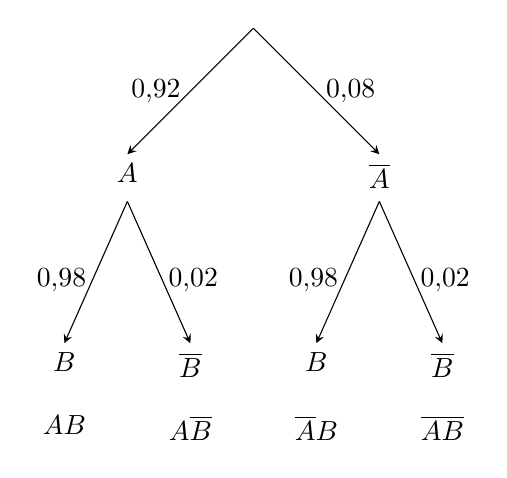
\begin{tikzpicture}[scale=.8,>=stealth]
				\coordinate [label=below:$A$](A) at (-2,-2);
				\coordinate [label=below:$\overline{A}$](B) at (2,-2);
				\coordinate [label=below:$B$](C) at (-3,-5);
				\coordinate [label=below:$\overline{B}$](D) at (-1,-5);
				\coordinate [label=below:$B$](E) at (1,-5);
				\coordinate [label=below:$\overline{B}$](F) at (3,-5);
				\draw[->](0,0)--(A);
				\draw[->](0,0)--(B);
				\draw[->](-2,-2.75)--(C);
				\draw[->](-2,-2.75)--(D);
				\draw[->](2,-2.75)--(E);
				\draw[->](2,-2.75)--(F);
				\coordinate [label=below:$AB$](G) at (-3,-6);
				\coordinate [label=below:$A\overline{B}$](H) at (-1,-6);
				\coordinate [label=below:$\overline{A} B$](I) at (1,-6);
				\coordinate [label=below:$\overline{A}\overline{B}$](J) at (3,-6);
				\draw (-1,-1) node[left] {$0{,}92$};
				\draw (1,-1) node[right] {$0{,}08$};
				\draw (-2.5,-4) node[left] {$0{,}98$};
				\draw (-1.5,-4) node[right] {$0{,}02$};
				\draw (1.5,-4) node[left] {$0{,}98$};
				\draw (2.5,-4) node[right] {$0{,}02$};
			\end{tikzpicture}
		\end{center}
		Theo sơ đồ hình cây ta có 
		\begin{itemize}
			\item Xác xuất để "Cả hai chuyến khởi hành đúng giờ" là
			$$\mathrm{P}(AB)=0{,}92\cdot 0{,}98=0{,}9016.$$
			\item Xác suất để "Có duy nhất một trong hai chuyến bay khởi hành đúng giờ" là
			$$\mathrm{P}(A\overline{B} \cup \overline{A}B)=0{,}92\cdot0{,}02+0{,}98\cdot 0{,}08=0{,}0968.$$
			\item   Xác suất để "Có ít nhất một trong hai chuyến khởi hành đúng giờ" là 
			$$P=1-\mathrm{P}(\overline{A}\overline{B})=1-0{,}08\cdot0{,}02=0{,}9984.$$
	\end{itemize}}
\end{ex}
\begin{ex}[\textit{Trích đề kiểm tra Toán 11 GKII - THPT NGUYỄN DU - NH24-25}]%[1D9H1-3]%[Dự án đề cương 3 Khối NH24-25-Dot 1-Nhật Thiện]
	Một bệnh truyền nhiễm có xác suất truyền bệnh là $0{,}2$ nếu tiếp xúc với người bệnh mà có đeo khẩu trang; là $0{,}7$ nếu tiếp xúc với người bệnh mà không đeo khẩu trang. Anh Nam tiếp xúc với một người bệnh hai lần, trong đó lần thứ nhất có đeo khẩu trang và lần thứ hai không đeo khẩu trang.
	\begin{enumerate}
		\item Tính xác suất anh Nam lần thứ nhất tiếp xúc không bị lây bệnh, lần thứ hai tiếp xúc bị lây bệnh.
		\item Tính xác suất anh Nam bị lây bệnh từ người bệnh mà anh tiếp xúc đó.
	\end{enumerate}
	\loigiai{
		Gọi $A$: "Lần thứ nhất tiếp xúc bị lây bệnh"; $B$: "Lần thứ hai tiếp xúc bị lây bệnh".
		\begin{enumerate}
			\item Xác suất anh Nam lần thứ nhất tiếp xúc không bị lây bệnh, lần thứ hai tiếp xúc bị lây bệnh là
			$$\mathrm{P}(\overline{A}B)=(1-0{,}2)\cdot 0{,}7=0{,}56.$$
			\item Xác suất anh Nam bị lây bệnh từ người bệnh mà anh tiếp xúc đó là
			$$1-\mathrm{P}(\overline{A}\overline{B})=1- (1-0{,}2)\cdot (1-0{,}7)=0{,}76.$$
		\end{enumerate}
	}
\end{ex}
\begin{ex}[Sách giáo  khoa Cánh diều]%[1C5B2-5]%[Dự án đề cương 3 Khối NH24-25-Dot 1-Nhật Thiện]
	Câu lạc bộ nghệ thuật của một trường trung học phổ thông gồm học sinh của cả ba khối $10, 11, 12$, mỗi khối có $5$ học sinh. Chon ngẫu nhiên $3$ học sinh để tham gia biểu diễn. Tính xác suất để $3$ học sinh được chọn chỉ thuộc hai khối.
	\loigiai{
		Mỗi cách chọn ra đồng thời $3$ học sinh trong câu lạc bộ cho ta một tổ hợp chập $3$ của $15$ phần tử.\\
		Do đó, không gian mẫu $\Omega$ gồm các tổ hợp chập $3$ của $15$ phần tử và $
		n(\Omega)=\mathrm{C}_{15}^3=\dfrac{15 !}{3 ! \cdot 12 !}=455$.\\
		Xét biến cố $A$: \lq\lq Chọn được $3$ học sinh chỉ thuộc hai khối\rq\rq.\\
		Sơ đồ hình cây biểu thị các khả năng thuận lợi cho biến cố $A$ như sau:\\
		\begin{tikzpicture}[font=\footnotesize, line join=round, line cap=round, >=stealth,scale=1.8]
			\path(0,0)node(a)[rectangle,draw=brown,text width=4cm,rounded corners=2mm,align=center]{Chọn $3$ học sinh chỉ ở hai khối}%Cấp 0
			++(-3.4,-1)node[rectangle,draw=brown,text width=3cm,rounded corners=2mm,align=center](b){Chọn $1$ học sinh lớp 10,\\ có 5 cách chọn}%Cấp 1
			(a)++(0,-1)node[rectangle,draw=brown,text width=3cm,rounded corners=2mm,align=center](d){Chọn $1$ học sinh lớp 11,\\ có 5 cách chọn}%Cấp 1
			(a)++(3.4,-1)node[rectangle,draw=brown,text width=3cm,rounded corners=2mm,align=center](c){Chọn $1$ học sinh lớp 12,\\ có 5 cách chọn}%Cấp 1
			;
			\path%Cấp 2 b
			(b)++(-0.8,-1.2)node[rectangle,draw=brown,text width=2cm,rounded corners=2mm,align=center](b1){Chọn $2$ học sinh lớp $11$, có $\mathrm{C}_{5}^2$ cách chọn}
			(b)++(0.8,-1.2)node[rectangle,draw=brown,text width=2cm,rounded corners=2mm,align=center](b3){Chọn $2$ học sinh lớp $12$, có $\mathrm{C}_{5}^2$ cách chọn}
			;
			\path%Cấp 3 b
			(b1)++(0,-1.2)node[rectangle,draw=brown,text width=2cm,rounded corners=2mm,align=center](b12){Có\\ $5\cdot \mathrm{C}_{5}^2=50$ cách chọn}
			;
			
			\path%Cấp 3 b
			(b3)++(0,-1.2)node[rectangle,draw=brown,text width=2cm,rounded corners=2mm,align=center](b32){Có\\ $5\cdot \mathrm{C}_{5}^2=50$ cách chọn}
			;
			%%%%%%%%%%%%%%%%%%%%%%%%%
			\path%Cấp 2 c
			(c)++(-0.8,-1.2)node[rectangle,draw=brown,text width=2cm,rounded corners=2mm,align=center](c1){Chọn $2$ học sinh lớp $10$, có $\mathrm{C}_{5}^2$ cách chọn}
			(c)++(0.8,-1.2)node[rectangle,draw=brown,text width=2cm,rounded corners=2mm,align=center](c3){Chọn $2$ học sinh lớp $11$, có $\mathrm{C}_{5}^2$ cách chọn}
			;
			
			\path%Cấp 3 c
			(c1)++(0,-1.2)node[rectangle,draw=brown,text width=2cm,rounded corners=2mm,align=center](c12){Có\\ $5\cdot \mathrm{C}_{5}^2=50$ cách chọn}
			;
			\path
			(c3)++(0,-1.2)node[rectangle,draw=brown,text width=2cm,rounded corners=2mm,align=center](c32){Có\\ $5\cdot \mathrm{C}_{5}^2=50$ cách chọn}
			;
			%%%%%%%%%%%%%%%%%%%%%%%%%%%%
			\path%Cấp 2 d
			(d)++(-0.8,-1.2)node[rectangle,draw=brown,text width=2cm,rounded corners=2mm,align=center](d1){Chọn $2$ học sinh lớp $10$, có $\mathrm{C}_{5}^2$ cách chọn}
			(d)++(0.8,-1.2)node[rectangle,draw=brown,text width=2cm,rounded corners=2mm,align=center](d3){Chọn $2$ học sinh lớp $12$, có $\mathrm{C}_{5}^2$ cách chọn}
			;
			
			\path%Cấp 3 d
			(d1)++(0,-1.2)node[rectangle,draw=brown,text width=2cm,rounded corners=2mm,align=center](d12){Có\\ $5\cdot \mathrm{C}_{5}^2=50$ cách chọn}
			;
			\path
			(d3)++(0,-1.2)node[rectangle,draw=brown,text width=2cm,rounded corners=2mm,align=center](d32){Có\\ $5\cdot \mathrm{C}_{5}^2=50$ cách chọn}
			;
			%Vẽ
			\draw[-stealth,teal,outer sep=0,inner sep=0](a.south)--++(-90:0.2)-|(b.north);
			\draw[-stealth,teal,outer sep=0,inner sep=0](a.south)--++(-90:0.2)-|(c.north);
			%%%
			\draw[-stealth,teal,outer sep=0,inner sep=0](a.south)--++(-90:0.2)-|(d.north);
			%%%
			\draw[-stealth,teal,outer sep=0,inner sep=0](b.south)--++(-90:0.1)-|(b1.north);
			%\draw[-stealth,teal,outer sep=0,inner sep=0](b.south)--++(-90:0.1)-|(b2.north);
			\draw[-stealth,teal,outer sep=0,inner sep=0](b.south)--++(-90:0.1)-|(b3.north);
			\draw[-stealth,teal,outer sep=0,inner sep=0](c.south)--++(-90:0.1)-|(c1.north);
			%\draw[-stealth,teal,outer sep=0,inner sep=0](c.south)--++(-90:0.1)-|(c2.north);
			\draw[-stealth,teal,outer sep=0,inner sep=0](c.south)--++(-90:0.1)-|(c3.north);
			\draw[-stealth,teal,outer sep=0,inner sep=0](d.south)--++(-90:0.1)-|(d3.north);
			\draw[-stealth,teal,outer sep=0,inner sep=0](d.south)--++(-90:0.1)-|(d1.north);
			%%%%%%%%%
			
			%\draw[-stealth,teal,outer sep=0,inner sep=0](b1.south)--++(-90:0.1)-|(b11.north);
			\draw[-stealth,teal,outer sep=0,inner sep=0](b1.south)--++(-90:0.1)-|(b12.north);
			%\draw[-stealth,teal,outer sep=0,inner sep=0](b2.south)--++(-90:0.1)-|(b21.north);
			%\draw[-stealth,teal,outer sep=0,inner sep=0](b2.south)--++(-90:0.1)-|(b22.north);
			%\draw[-stealth,teal,outer sep=0,inner sep=0](b3.south)--++(-90:0.1)-|(b31.north);
			\draw[-stealth,teal,outer sep=0,inner sep=0](b3.south)--++(-90:0.1)-|(b32.north);
			
			%\draw[-stealth,teal,outer sep=0,inner sep=0](c1.south)--++(-90:0.1)-|(c11.north);
			\draw[-stealth,teal,outer sep=0,inner sep=0](c1.south)--++(-90:0.1)-|(c12.north);
			%\draw[-stealth,teal,outer sep=0,inner sep=0](c2.south)--++(-90:0.1)-|(c21.north);
			%\draw[-stealth,teal,outer sep=0,inner sep=0](c2.south)--++(-90:0.1)-|(c22.north);
			%\draw[-stealth,teal,outer sep=0,inner sep=0](c3.south)--++(-90:0.1)-|(c31.north);
			\draw[-stealth,teal,outer sep=0,inner sep=0](c3.south)--++(-90:0.1)-|(c32.north);
			%%%
			\draw[-stealth,teal,outer sep=0,inner sep=0](d3.south)--++(-90:0.1)-|(d32.north);
			\draw[-stealth,teal,outer sep=0,inner sep=0](d1.south)--++(-90:0.1)-|(d12.north);
			
		\end{tikzpicture}\\
		\\
		%%%%%%%%%%%%%%%%%
		\noindent Như vậy, số kết quả thuận lợi cho biến cố $A$ là $n(A)=50 \cdot 6=300$.\\
		Vậy xác suất của biến cố $A$ là $\mathrm{P}(A)=\dfrac{n(A)}{n(\Omega)}=\dfrac{300}{455}=\dfrac{60}{91}$.}
\end{ex}
\begin{ex}%[1C5B2-6]%[Dự án đề cương 3 Khối NH24-25-Dot 1-Nhật Thiện]
	Hai bạn Mai và Thi cùng tham gia một kì kiểm tra ngoại ngữ một cách độc lập nhau. Xác suất để bạn Mai và bạn Thi đạt từ điểm $7$ trở lên lần lượt là $0{,}8$ và $0{,}9$. Tính xác suất của biến cố $C$: "Cả hai bạn đều đạt từ điểm $7$ trở lên".
	\loigiai{
		Xét biến cố $A\colon$"Bạn Mai đạt từ điểm $7$ trở lên", ta có $\mathrm{P}(A)=0{,}8$.\\
		Xét biến cố $B\colon$"Bạn Thi đạt từ điểm $7$ trở lên", ta có $\mathrm{P}(B)=0{,}9$.\\
		Ta thấy $A,B$ là hai biến cố độc lập và $C=A \cap B$, suy ra 
		$\mathrm{P}(C)=\mathrm{P}(A) \cdot \mathrm{P}(B)=0{,}8 \cdot 0{,}9=0{,}72$.
	}
\end{ex}
\begin{ex}%[1D9H1-3]%[Dự án đề cương 3 Khối NH24-25-Dot 1-Nhật Thiện]
	Một đề kiểm tra $5$ phút có hai câu trắc nghiệm. Biết xác suất đúng mỗi câu là $0{,}25$. Tính xác suất để một học sinh không học bài có thể khoang đúng được cả hai câu.
	\loigiai{
		Gọi xác suất để học sinh khoanh đúng hai câu hỏi lần lượt là $\mathrm{P}(A)=\mathrm{P}(B)=0{,}25$.\\
		Vì mỗi biến cố là độc lập với nhau nên ta có xác suất cần tìm là $\mathrm{P}(AB)=0{,}25\cdot 0{,}25=0{,}0625$.
	}
\end{ex}

\begin{ex}%[1D9H1-3]%[Dự án đề cương 3 Khối NH24-25-Dot 1-Nhật Thiện]
	Hai đội công nhân trong một nhà máy sản xuất có xác suất tạo ra sản phẩm tốt lần lượt là $0{,}75$ và $0{,}85$. Tính xác suất phế phẩm mà nhà máy đó tạo ra bởi cả hai đội.
	\loigiai{
		Gọi xác suất tạo ra sản phẩm tốt của hai đội công nhân lần lượt là $\mathrm{P}(A)=0{,}75$ và $\mathrm{P}(B)=0{,}85$.\\
		Gọi xác suất tạo ra phế phẩm của hai đội công nhân lần lượt là $\mathrm{P}(\overline{A})=0{,}25$ và $\mathrm{P}(\overline{B})=0{,}15$.\\
		Vậy xác suất phế phẩm mà nhà máy đó tạo ra bỏi cả hai đội là
		$$\mathrm{P}\left(\overline{A}\cap \overline{B}\right)=0{,}25\cdot 0{,}15=0{,}0375.$$
	}
\end{ex}

\begin{ex}%[1D9H1-3]%[Dự án đề cương 3 Khối NH24-25-Dot 1-Nhật Thiện]
	Hai bạn An và Minh cùng tham gia giải cờ vua cấp tỉnh. Biết rằng hai bạn không ở chung $1$ bảng và mỗi bảng chỉ có một người vô vòng chung kết. Biết xác suất vô vòng chung kết của An và Minh lần lượt là $0{,}35$ và $0{,}45$. Tính xác suất để An và Minh cùng vô vòng chung kết.
	\loigiai{
		Gọi xác suất để An và Minh vô vòng chung kết lần lượt là $\mathrm{P}(A)=0{,}35$ và $\mathrm{P}(B)=0{,}45$.\\
		Vậy xác suất để cả hai bạn cùng vô vòng chung kết là $\mathrm{P}(AB)=0{,}35\cdot 0{,}45=0{,}1575$.
	}
\end{ex}

\begin{ex}%[1D9H1-3]%[Dự án đề cương 3 Khối NH24-25-Dot 1-Nhật Thiện]
	Một nhà máy có hai tổ máy sản xuất một mặt hàng, biết rằng xác suất để hai tổ máy phải nghỉ để bảo dưỡng lần lượt là $0{,}2$ và $0{,}32$. Tính xác suất để cả hai tổ máy đều hoạt động.
	\loigiai{
		Gọi xác suất để hai tổ máy phải nghỉ để bảo dưỡng lần lượt là $\mathrm{P}(A)=0{,}2$ và $\mathrm{P}(B)=0{,}32$.\\
		Nên xác suất để hai tổ máy đều hoạt động là $\mathrm{P}(\overline{A})=0{,}8$ và $\mathrm{P}(\overline{B})=0{,}68$.\\
		Vậy xác suất để cả hai tổ máy đều hoạt động là $\mathrm{P}\left(\overline{A}\cap \overline{B}\right)=0{,}8\cdot 0{,}68=0{,}544$.
	}
\end{ex}